\chapter{ISRU \& Buoyancy Subsystem}\label{chap:ISRU}

% Required packages if not already included in the preamble:
% \usepackage[table]{xcolor}
% \usepackage{tabularx}
% \usepackage{array}
% \usepackage{float}

% If these colours are already defined elsewhere, do not define them twice.
\definecolor{scorefive}{HTML}{B7E1CD}
\definecolor{scorefour}{HTML}{D9EAD3}
\definecolor{scorethree}{HTML}{FCE5CD}
\definecolor{scoretwo}{HTML}{F4CCCC}
\definecolor{scoreone}{HTML}{E6B8AF}

\section{Balloon Design Options Trade-Off}
\label{sec:balloon_design_options_tradeoff}

The design option tree resulted in three straw-man concepts for the lifting and altitude control \cite{baseline_vista}. These concepts were compared to determine whether they are feasible, and to determine which of them would be the most optimal in terms of balloon sizing, gas-processing system, deployment sequence, power demand, reliability, operational complexity, and long-term feasibility. For that, the trade-off has been performed.

\textbf{Option 1:} A large balloon, initially partially filled with helium, and filled with in situ obtained nitrogen over a long period of time, utilising atmospheric CO$_2$ as ballast for altitude control.

\textbf{Option 2:} A filled nitrogen balloon, in situ nitrogen for top-up, altitude controlled using an internal superpressure bladder.

\textbf{Option 3:} A nitrogen balloon, arriving at Venus empty, utilising an internal superpressure bladder for altitude control. A temporary, disposable helium balloon whose purpose is to give the in situ nitrogen extractor enough time to fill the primary balloon.

These are the three options identified and selected in the baseline concept selection. The main mission drivers include the in situ resource utilisation (ISRU) for leakage compensation, power of 500 Wh and total aerobot mass. A full numerical sizing and power estimation have only been developed for Option 2 at this stage. Therefore, the trade-off will be performed using semi-quantitative methods, which still help to clearly establish which concept is the most optimal for the mission purpose. Numerical values for Option 2 will be used where available, such as nitrogen leakage replacement rate, continuous equivalent ISRU power, and altitude-control pump power. For Options 1 and 3, the scores are based on architecture-level metrics that can be evaluated without a full model.

\subsection{Trade-Off Criteria and Weights}
\label{subsec:balloon_trade_criteria}

The selection criteria are selected to match those used in system engineering, such as performance, mass, power, risk, reliability, cost/schedule and sustainability. The criteria, weights, and explanation are shown in Table~\ref{tab:balloon_trade_criteria}.

\begin{table}[H]
\centering
\caption{Balloon design option trade-off criteria and weights.}
\label{tab:balloon_trade_criteria}
\footnotesize
\renewcommand{\arraystretch}{1.12}
\setlength{\tabcolsep}{5pt}
\begin{tabularx}{\textwidth}{@{}p{0.36\textwidth} c X@{}}
\toprule
\textbf{Criterion} & \textbf{Weight} & \textbf{Explanation} \\
\midrule
C1 -- Long-duration lifting robustness 
& 20\%  
& How well can a concept maintain lift for 5 years. \\

C2 -- Power consumption feasibility 
& 20\% 
& Expected gas-processing and altitude-control energy demand. Has to comply with the 500 Wh constraint. \\

C3 -- Deployment and early mission operation risk 
& 15\% 
& Number of potential critical events before stable operation, and to what extent stable operation depends on early ISRU performance. \\

C4 -- Altitude control 
& 15\%  
& Whether the aerobot can maintain and change altitude without losing the lifting gas. \\

C5 -- System complexity 
& 15\%  
& Number of active components such as valves, sensors, pumps, actuators etc. \\

C6 -- Mass and packaging feasibility 
& 10\%  
& Whether the entire system complies with mass constraints. \\

C7 -- Sustainability 
& 5\%  
& Contamination risk. \\
\midrule
\textbf{Total} & \textbf{100\%} & \\
\bottomrule
\end{tabularx}
\end{table}

The weights are chosen as follows, as C1 and C2 are the hardest ones to fulfil. There is not enough representative data about the Venus atmosphere and how it affected the previous missions for prolonged periods of time. C2, on the other hand, is weighted heavily, as the 500 Wh requirement is very strict, and the system must pump and separate kilograms of atmosphere per day for 5 years, meaning it will consume a substantial amount of power. C3, C4 and C5 have been weighted slightly less, as these requirements are slightly clearer, and can be backed up by earlier missions and relevant data. C6 is weighted 0.1, as the system itself is not particularly heavy due to use of advanced materials and hardware, making it less critical. Finally, sustainability is only relevant during the manufacturing process and the end of life, which can also be taken care of later.



\subsection{Trade-Off Table}
\label{subsec:balloon_trade_table}

The final weighted score is calculated as $S_{\mathrm{weighted}} = \sum_i w_i S_i$, where $w_i$ is the criterion weight and $S_i$ is the assigned score between 1 and 5.

The trade-off table is shown in Table~\ref{tab:balloon_tradeoff_table}.

\begin{table}[H]
\centering
\caption{Balloon design options trade-off table.}
\label{tab:balloon_tradeoff_table}
\footnotesize
\renewcommand{\arraystretch}{1.12}
\setlength{\tabcolsep}{5pt}
\begin{tabularx}{\textwidth}{@{}X c c c c@{}}
\toprule
\textbf{Criterion} & \textbf{Weight} & \textbf{Option 1} & \textbf{Option 2} & \textbf{Option 3} \\
\midrule
C1 -- Long-duration lifting robustness 
& 20\% 
& \cellcolor{scorethree}3 
& \cellcolor{scorefive}5 
& \cellcolor{scorethree}3 \\

C2 -- Power consumption feasibility 
& 20\% 
& \cellcolor{scoretwo}2 
& \cellcolor{scorefour}4 
& \cellcolor{scoreone}1 \\

C3 -- Deployment and early mission operation risk 
& 15\%  
& \cellcolor{scorethree}3 
& \cellcolor{scorefive}5 
& \cellcolor{scoretwo}2 \\

C4 -- Altitude control 
& 15\%  
& \cellcolor{scorethree}3 
& \cellcolor{scorefive}5 
& \cellcolor{scorefour}4 \\

C5 -- System complexity 
& 15\%  
& \cellcolor{scorethree}3 
& \cellcolor{scorefour}4 
& \cellcolor{scoretwo}2 \\

C6 -- Mass and packaging feasibility 
& 10\% 
& \cellcolor{scorefour}4 
& \cellcolor{scorethree}3 
& \cellcolor{scorethree}3 \\

C7 -- Sustainability 
& 5\%  
& \cellcolor{scorethree}3 
& \cellcolor{scorefour}4 
& \cellcolor{scoretwo}2 \\
\midrule
\textbf{Total} 
& \textbf{100\%} 
& \textbf{2.90} 
& \textbf{4.40} 
& \textbf{2.40} \\
\bottomrule
\end{tabularx}
\end{table}

\subsection{Score Justification}
\label{subsec:balloon_score_justification}

\textbf{Option 1} scores a decent but not high score of 2.90. It is advantageous as it uses helium initially to keep the balloon afloat, so it does not need to be filled with N$_2$ by the ISRU system immediately after deployment. However, it relies on a gradual transition from helium to nitrogen. Using the power consumption estimation script, at an altitude of 55 km, the system needs a total of approximately 300 kg of nitrogen to stay afloat, split between the superpressure balloon and zero-pressure balloon. To fill it with nitrogen in days, around 5 kg of N$_2$ would need to be pumped per day. According to the preliminary power consumption estimates, this would require about 993.4 W of power during the filling phase, which is not feasible with the 500 Wh energy storage budget unless the filling process is spread over a much longer period. This would decrease the useful mission time.

On top of that, it requires CO$_2$ ballast for altitude control, which adds complexity and creates a more consumable-based control approach. Therefore, it scores lower in system complexity (C5) and altitude-control capability (C4). It scores well in mass and packaging feasibility, as it is only one balloon without extra add-ons.

\textbf{Option 2} scores the highest, with a final score of 4.40. Its main advantage is its simplicity and the fact that it reaches its stable long-term configuration immediately after deployment, as it already contains the nitrogen. The ISRU system is only required for leakage compensation, which, based on the leakage estimation script, is around 185 grams per day as can be seen in \autoref{tab:n2_leakage_summary}. This means that the continuous power consumption of the entire system is about 54 W at maximum leakage rate, according to \autoref{tab:isru_power_results}. This reduces the dependency on early ISRU performance, making the concept more robust for long-duration operation.

Altitude control is performed by means of a superpressure bladder inside the zero-pressure balloon, which is favourable since superpressure volumes provide passive altitude stability. Pumping between pressure volumes is also a known method for changing buoyancy in variable-altitude balloon concepts, which have already been tested before.

It scores lower in mass and packaging, as, for example, to deploy at a 55 km altitude, roughly 300 kg of nitrogen is required, which needs to be brought all the way to Venus. However, this is compensated by the other criteria, making this concept clearly the best choice.

\textbf{Option 3} scores poorly overall, with a final score of 2.40. Despite being a valid concept, it clearly loses on power consumption for the same reason as Option 1, since the main nitrogen balloon still needs to be filled after arrival. It also loses on criteria C3 and C5, as having an extra balloon increases system complexity and adds more risks during deployment and early operation. Moreover, an extra balloon is worse for sustainability, as there will be more material to dispose of at the end of life.

Its altitude-control mechanism concept is reasonable once the main balloon is filled up, but the early-operation risk still dominates the trade-off. Therefore, Option 3 is not selected.

Based on the weighted trade-off, Option 2 is selected as the preferred baseline architecture. Although it has a mass and packaging disadvantage, it provides the best overall balance between long-duration lifting robustness, deployment risk, altitude-control capability and operational simplicity. The selected concept is therefore a filled nitrogen balloon with in situ nitrogen top-up for leakage compensation and an internal superpressure bladder for altitude control.



\definecolor{scorefive}{HTML}{B7E1CD}
\definecolor{scorefour}{HTML}{D9EAD3}
\definecolor{scorethree}{HTML}{FCE5CD}
\definecolor{scoretwo}{HTML}{F4CCCC}
\definecolor{scoreone}{HTML}{E6B8AF}

\section{\texorpdfstring{N$_2$ Separation System Trade-Off}{N2 Separation System Trade-Off}}
\label{sec:n2_separation_tradeoff}

The nitrogen separation system is required to extract N$_2$ from the Venus atmosphere for leakage compensation. Three main methods were considered for the trade-off:

\begin{enumerate}
    \item \textbf{PSA/Molecular Sieve:} uses selective adsorption beds to remove CO$_2$-rich gas and produce an N$_2$-enriched stream. The beds are regenerated by pressure swing.
    \item \textbf{Cryotrapping:} cools the atmospheric feed so that CO$_2$ is frozen out, leaving a more N$_2$-enriched gas stream.
    \item \textbf{Chemical Getters:} uses reactive material to chemically bind or remove CO$_2$, leaving N$_2$ behind.
\end{enumerate}

The considered trade-off criteria are system mass, complexity, power, reliability and Venus environment compatibility. These are selected because the separation system must survive the full mission, fit within the power and mass budget, and operate in the acidic Venus atmosphere.

\subsection{Trade-Off Criteria and Weights}
\label{subsec:n2_trade_criteria}

The criteria, weights, and explanation are shown in Table~\ref{tab:n2_trade_criteria}. Reliability and power are given the highest weights, since failure of the separation system would threaten the whole mission and the onboard energy storage is strongly limited.

\begin{table}[H]
\centering
\caption{N$_2$ separation system trade-off criteria and weights.}
\label{tab:n2_trade_criteria}
\footnotesize
\renewcommand{\arraystretch}{1.12}
\setlength{\tabcolsep}{5pt}
\begin{tabularx}{\textwidth}{@{}p{0.30\textwidth} c X@{}}
\toprule
\textbf{Criterion} & \textbf{Weight} & \textbf{Explanation} \\
\midrule
Reliability 
& 25\% 
& Failure of the separation system will threaten the entire mission. \\

Power 
& 25\%  
& Limited onboard energy storage. \\

Mass 
& 20\%  
& The separation system must fit within a mass budget. \\

Venus Environment 
& 15\%  
& The separation system must survive the acidic atmosphere. \\

Complexity 
& 15\%  
& Affects testing, integration, and increases the number of potential points of failure. \\
\midrule
\textbf{Total} & \textbf{100\%} & \\
\bottomrule
\end{tabularx}
\end{table}

\subsection{Trade-Off Table}
\label{subsec:n2_trade_table}

The final weighted score is calculated as $S_{\mathrm{weighted}} = \sum_i w_i S_i$, where $w_i$ is the criterion weight and $S_i$ is the assigned score.

The trade-off table is shown in Table~\ref{tab:n2_tradeoff_table}. The scores are assigned from 1 to 5, where 5 is the best score.

\begin{table}[H]
\centering
\caption{N$_2$ separation system trade-off table.}
\label{tab:n2_tradeoff_table}
\footnotesize
\renewcommand{\arraystretch}{1.12}
\setlength{\tabcolsep}{5pt}
\begin{tabularx}{\textwidth}{@{}X c c c c c c@{}}
\toprule
\textbf{Method} & \textbf{Reliability} & \textbf{Power} & \textbf{Mass} & \textbf{Venus Env.} & \textbf{Complexity} & \textbf{Total} \\
& \textbf{25\%} & \textbf{25\%} & \textbf{20\%} & \textbf{15\%} & \textbf{15\%} & \\
\midrule
PSA/Molecular Sieve 
& \cellcolor{scorefour}4 
& \cellcolor{scorethree}3 
& \cellcolor{scorefour}4 
& \cellcolor{scoretwo}2 
& \cellcolor{scorethree}3 
& \textbf{3.30} \\

Cryotrapping 
& \cellcolor{scoretwo}2 
& \cellcolor{scoreone}1 
& \cellcolor{scoretwo}2 
& \cellcolor{scoretwo}2 
& \cellcolor{scoretwo}2 
& \textbf{1.75} \\

Chemical Getters 
& \cellcolor{scorethree}3 
& \cellcolor{scorefour}4 
& \cellcolor{scoreone}1 
& \cellcolor{scoretwo}2 
& \cellcolor{scorefour}4 
& \textbf{2.85} \\
\bottomrule
\end{tabularx}
\end{table}

\subsection{Score Justification}
\label{subsec:n2_score_justification}

\textbf{PSA/Molecular Sieve} receives the highest score. Its main advantage is that it is a regenerable separation method, meaning that the adsorbent beds can be reused, instead of carrying a large consumable mass. PSA/molecular sieves are also a known technology, which has strong industrial heritage, therefore scoring high in reliability. It is not a passive system in terms of power, since valves operation and feed compression are required, which also increases the complexity. However, it is still much less power-consuming and less complex compared to cryotrapping. The Venus environment score is moderate because the sieve beds must still be protected from sulfuric acid aerosols by filters or inlet protection. Finally, the mass score is relatively high compared to chemical getters and cryotrapping, since PSA avoids a large consumable mass and does not require a full cooling system.

\textbf{Cryotrapping} receives the lowest score. First, its main disadvantages are power consumption and mass. Since it needs to constantly cool a large amount of gas, it would require a cryocooler, heat exchangers, insulation and thermal rejection hardware, making it highly demanding in both power and mass, as well as increasing system complexity, which also reduces the score. It also scores poorly in Venus environment compatibility for the same reason as PSA, as sulfuric acid aerosols and contaminants can deposit on cold surfaces or worsen clogging.

\textbf{Chemical getters} receive a moderate score. Their main advantage is simplicity. Power consumption is much lower compared to PSA and cryotrapping, hence it scores well in both power and system complexity. This advantage however only holds when the getter is treated as a consumable, meaning major mass concerns will arise. Since N$_2$ is only 3.5\% of the atmosphere, the CO$_2$ mass that must be removed is roughly:
\begin{align}
    \frac{m_{\mathrm{CO_2}}}{m_{\mathrm{N_2}}}
    =
    \frac{0.965 \cdot 44}{0.035 \cdot 28}
    \approx 43
\end{align}
Therefore, for 185 grams of N$_2$, about 8 kg of CO$_2$ must be removed daily, which corresponds to over 14 tonnes of CO$_2$ over a 5-year mission duration. This makes the technology infeasible from a mass point of view. On the other hand, if the getter were made regenerable, it would lose much of its simplicity and would require extra power and regeneration hardware, making it closer to PSA but with less heritage.


Based on the weighted trade-off, PSA/Molecular Sieve is selected as the preferred nitrogen separation method. Although it is not passive and still requires valves, a feed compressor and inlet protection, it provides the best overall balance between reliability, power, mass, complexity and Venus environment compatibility.

\section{Balloon Material Options Trade-Off}

\noindent The balloon envelope is the most operationally sensitive structural element of the VISTA aerobot. Unlike terrestrial or even stratospheric balloon envelopes, the Venus cloud-layer environment simultaneously imposes several requirements that no single polymer film can satisfy individually \cite{yung2024planetaryvenus}. The outer surface must resist concentrated sulphuric acid aerosols H$_2$SO$_4$ \cite{delitsky2023cloudchemistryvenus}, the gas-barrier layer must suppress nitrogen leakage over a five-year float duration, the load-bearing layer must sustain superpressure-driven hoop stresses at 55\,km altitude, and every component must remain mechanically sound through interplanetary cruise, deployment shock, and multi-year thermal cycling \cite{Hall2007_VenusPrototype,Hall2009_SecondGen,Hall2011_TechDev}. 
\medskip

\noindent This chapter presents the material trade-off analysis and refilling mechanism selection process for the VISTA balloon dome. Section \ref{sec:operational-and-req} characterises the environmental loads and derives the material-level requirements. Section \ref{sec:mat-candidates} reviews the candidate materials at the individual film level, covering acid resistance, gas permeability, tensile properties, density, and brittleness at operational conditions. Section \ref{sec:mat-architectures} extends the analysis to multi-layer laminate architectures that might combine desired properties. Section \ref{sec:mat-tradeoff} presents the scored trade-off and section \ref{sec:mat-selection} states the selected architecture and justifies the selection against the mission constraints.

\section{Operational Conditions and Requirements}\label{sec:operational-and-req}

First, the operational environment must be revisited. Then, its take-aways will be used to express subsystem-specific requirements flowing down from system-level VISTA requirements \cite{baseline_vista}.

\subsection{Environmental Loads at the Float Altitude}
\label{sec:mat-environment}

The VISTA float altitude of approximately 55\,km sits within the main Venusian cloud layer. The relevant environmental parameters for envelope material selection are summarised in Table \ref{tab:float-environment}. At this altitude, the atmospheric temperature is approximately 27-37\,$^\circ$C and the pressure is approximately 0.4-0.5\,bar. These conditions are mild in comparison to the Venus surface, but the sulphuric acid environment is uniquely aggressive: cloud droplets of H$_2$SO$_4$ are present continuously at 49-57\,km \cite{Knollenberg1980_VenusAerosol}. During descent and inflation, the envelope may encounter higher acid concentrations and steeper temperature gradients that also have to be accounted for. The design must also consider solar UV irradiance on the dayside, which is relevant to materials with photosensitive bond chemistry.

\begin{table}[H]
\centering
\caption{Environmental parameters at the VISTA float altitude (55\,km) relevant to envelope material selection.}
\label{tab:float-environment}
\footnotesize
\renewcommand{\arraystretch}{1.15}
\setlength{\tabcolsep}{5pt}
\begin{tabularx}{\linewidth}{@{}p{3.35cm} p{2.6cm} X@{}}
\toprule
\textbf{Parameter} & \textbf{Value} & \textbf{Design significance} \\
\midrule
Temperature & 27-37\,$^\circ$C & Within polymer service range; critical for acid reaction kinetics. \\
Pressure & $\approx$0.46\,bar & Superpressure differential $\Delta p \approx$2-4\,kPa drives hoop stress. \\
H$_2$SO$_4$ concentration & 75-85\,wt\% & Attacks polyesters, polyamides, and most non-fluorinated organics. \\
H$_2$SO$_4$ exposure duration & $\geq$5 years continuous & Eliminates short-term acid-resistant coatings; requires inherently inert chemistry. \\
Dayside UV & $\sim$3$\times$ terrestrial & Degrades UV-sensitive polymer chains. \\
Night temperature swing & $\pm$20\,$^\circ$C per cycle & Drives thermal fatigue in laminates with mismatched CTE. \\
Lifting gas & Nitrogen (in situ) & Lower permeability kinetic diameter (0.364\,nm) than H$_2$ (0.289\,nm) \cite{PolyimideGasTransport2024}. \\
Float duration & $\geq$5 years & $\approx$365 atmospheric circumnavigation cycles; $\approx$1825 days of acid exposure. \\
\bottomrule
\end{tabularx}
\end{table}

\noindent One important design consequence of the nitrogen-ISRU architecture is that the driver for leaking considerations is nitrogen permeability through the envelope, not helium permeability as in the JPL helium-based prototypes \cite{Hall2007_VenusPrototype,Hall2009_SecondGen}. Because the kinetic diameter of N$_2$ (0.364\,nm) is larger than that of He (0.26\,nm) or H$_2$ (0.289\,nm), nitrogen permeates through most polymer films at a substantially lower rate than noble helium or small-diameter dihydrogen molecules. This is a structural advantage of the VISTA nitrogen architecture from a material perspective. Mainly, laminates that failed to contain helium over months may retain nitrogen for multi-year operation, and materials that were proven in retaining helium will provide a reliability margin for a less constraining in this regard nitrogen-based design \cite{Sebok2015_PTFEpermeability}.

\subsection{Derived Material-Level Requirements}
\label{sec:mat-requirements}

From the top-level mission requirements (Baseline Review \cite{baseline_vista} and the environmental characterisation above, the following material-level derived requirements are identified for the balloon envelope:

\begin{table}[H]
\centering
\small
\caption{Envelope Material Requirements}
\begin{tabular}{|l|p{3.5cm}|p{9cm}|}
\hline
\textbf{ID} & \textbf{Name} & \textbf{Requirement Statement} \\ \hline

REQ-MAT-01 & Acid resistance & The outer surface shall exhibit no measurable loss of mechanical integrity after 5-year continuous exposure to operational H$_2$SO$_4$ concentration at 55 km above the Venusian surface. \\ \hline

REQ-MAT-02 & Nitrogen gas retention & The total envelope nitrogen permeance shall be such that the steady-state leakage loss can be replaced by the in situ nitrogen replenishment system at a rate consistent with the power budget allocation to the ISRU subsystem. \\ \hline

REQ-MAT-03 & Tensile strength & The envelope areal tensile load capacity shall provide a safety factor of $\geq 3$ against the worst-case superpressure burst load of $\Delta p \approx 39{,}200\,\mathrm{Pa}$ for a sphere of radius $R$, where the hoop stress is $\sigma = \Delta p \cdot R / (2t)$ \cite{Hall2007_VenusPrototype}. \\ \hline

REQ-MAT-04 & Areal mass density & The envelope areal density $\sigma$ shall not exceed 150\,g/m$^2$ for the nominal design case. \\ \hline

REQ-MAT-05 & Non-brittleness and flex tolerance & The material shall survive the stowed and packaged configuration during launch and the aerial deployment without pinhole formation or delamination. This implies a minimum elongation at break of $\geq 2\%$ and a minimum flex fatigue life of 1000 cycles without loss of gas-barrier integrity. \\ \hline

REQ-MAT-06 & UV and thermal stability & The material shall retain $\geq 80\%$ of its initial tensile strength after 5 years of dayside UV exposure at Venus irradiance levels and after 1825 diurnal temperature cycles of $\pm 40\,^\circ$C amplitude. \\ \hline

REQ-MAT-07 & TRL & All constituent materials shall have a TRL of at least 4 in relevant environments, aligned with project's general TRL floor. \\ \hline

\end{tabular}
\label{tab:material_requirements}
\end{table}


\iffalse
\section{Individual Candidate Material Assessment}
\label{sec:mat-candidates}

The candidate materials are assessed here at the individual film or fabric level before combined laminate architectures are constructed in Section \ref{sec:mat-architectures}. Each candidate is evaluated against the six material-level criteria: acid resistance, N$_2$ gas permeability, tensile strength per unit areal density, brittleness, UV and thermal stability, and heritage/TRL. An effort was made to rely on available quantitative data, but if only relative comparisons are available from the Venus aerobot literature, the rating is qualitative.


\subsection{Polytetrafluoroethylene (PTFE) Film}
\label{ssec:ptfe}

PTFE was the outer layer of the original Vega balloon envelopes, where it demonstrated flight-proven acid resistance at the Venus cloud level \cite{Kremnev1986}. Its fully fluorinated carbon backbone renders it essentially inert to sulphuric acid, and the material shows no measurable degradation in tensile properties after immersion in H$_2$SO$_4$ present in Vanusian clouds \cite{FosterMiller1996_PBOVenus}. PTFE is also chemically stable under the UV spectrum relevant to Venus.

\begin{figure}[H]
    \centering
    
\includegraphics[width=0.18\linewidth]{fig/PTFE.png}
    \caption{Molecular Structure of PTFE}
    \label{fig:PTFE}
\end{figure}

\noindent The gas permeability of a 0.1\,mm PTFE membrane has been quantitatively characterised by Seb\"{o}k et al., who report that H$_2$ permeability through PTFE is substantially higher than N$_2$ permeability: the diffusivity ranking shows $D_{H_2} \gg D_{N_2}$ across the range from room temperature to 180\,$^\circ$C, which is consistent with difference in kinetic diameters of considered molecules (N$_2$ has a kinetic diameter of 0.364\,nm versus H$_2$ at 0.289\,nm) \cite{Sebok2015_PTFEpermeability}. For the VISTA nitrogen-ISRU architecture this is favourable, as it proves N$_2$ permeates through PTFE at a substantially lower rate than H$_2$ would under identical conditions - once again highlighting the reliability margin of helium permeability findings, mentioned in Section \ref{sec:mat-environment}. Moreover, comparative fluoropolymer gas permeability data place PTFE nitrogen permeability at $\sim$10\,cm$^3$/m$^2$/d/bar, substantially lower than PFA (500\,cm$^3$/m$^2$/d/bar) or FEP (1200\,cm$^3$/m$^2$/d/bar) at the same thickness \cite{PCTFE_Permeability_Guide}.

\medskip

\noindent This laminate is not without its weaknesses, though. PTFE film is mechanically weak when unsupported. It has a relatively low tensile strength (20-35\,MPa depending on sintering condition) and does not withstand repetitive folding without developing microcrack networks \cite{FEPwiki}. It cannot be melt-processed and therefore cannot be heat-seamed, which is a practical limitation for gore-seam construction of the balloon dome \cite{FluorocarbonPTFEvsPFA}. PTFE film is therefore best used as an outer protective layer and not as the primary structural element.

\subsection{Perfluoroalkoxy Polymer (PFA) Film}
\label{ssec:pfa}

PFA shares PTFE's fully fluorinated chemistry (see Figure \ref{fig:PFA}) and therefore its good acid resistance, but has an advantage of being melt-processible and heat-welded \cite{FluorocarbonPTFEvsPFA}. This makes it more practical for seam construction than PTFE film. JPL specifically proposed PFA as an alternative protective outer-layer fluoropolymer for Venus aerobot applications \cite{FosterMiller1996_PBOVenus}. Its continuous service temperature extends to approximately 260\,$^\circ$C, well above the Venus cloud-level conditions.

\begin{figure}[H]
    \centering
    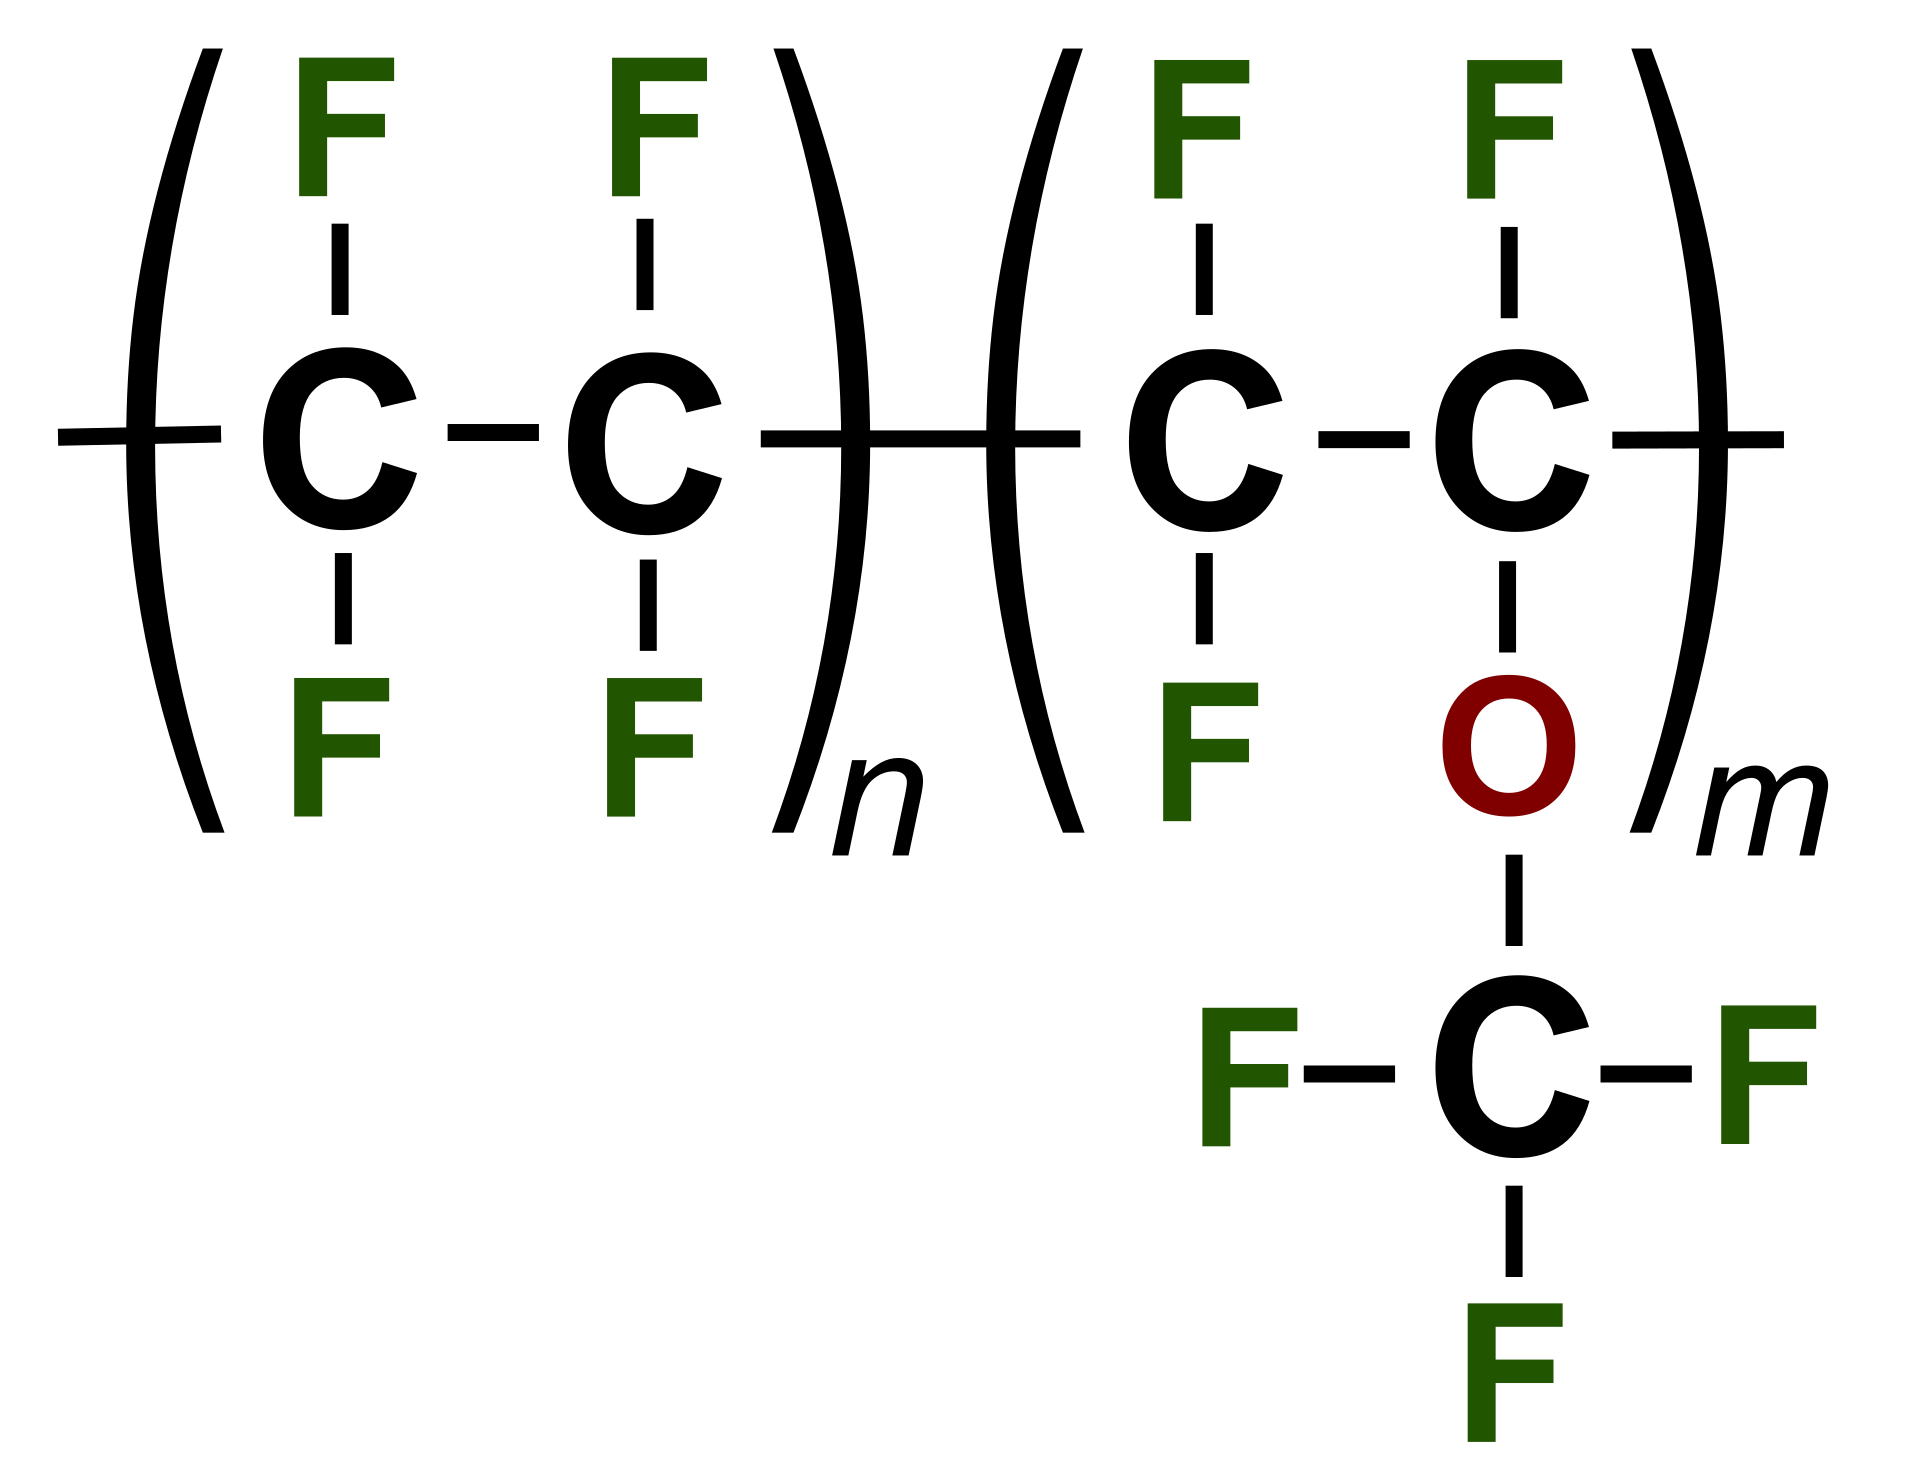
\includegraphics[width=0.25\linewidth]{fig/PFA.png}
    \caption{Molecular Structure of PFA}
    \label{fig:PFA}
\end{figure}

\noindent PFA's N$_2$ permeability is higher than PTFE at the same thickness, due to PFA's lower crystallinity and larger free volume within the polymer matrix \cite{PCTFE_Permeability_Guide,FEP_PFA_permeability}. In a gas-barrier role, PFA is therefore inferior to PTFE, though it still outperforms polyimide films by roughly an order of magnitude. PFA's tensile strength is similar to PTFE (25-30\,MPa), and it is likewise not usable as a structural load-bearing layer without a fabric substrate. Its flex life is better than sintered PTFE due to the melt-processible microstructure. Therefore, whether PTFE or PFA will be used will largely depend on combination of other materials in the multi-layer architectures considered, and what remaining parameters will be of highest importance for successful combined performance.


\subsection{Fluorinated Ethylene Propylene (FEP) Film}
\label{ssec:fep}

FEP was the outer layer of the first JPL Venus balloon prototype \cite{Hall2007_VenusPrototype}. It is chemically similar to PTFE and PFA, as shown in the Figure \ref{fig:FEP}, and melts at approximately 260\,$^\circ$C, enabling film extrusion and heat-seaming. FEP is slightly softer than PTFE and does not withstand repetitive folding as well \cite{FEPwiki}. Its N$_2$ permeability is at approximately 1200\,cm$^3$/m$^2$/d/bar, making it a weaker gas barrier than both PTFE and PFA at equivalent thickness \cite{PCTFE_Permeability_Guide}. 

\begin{figure}[H]
    \centering
    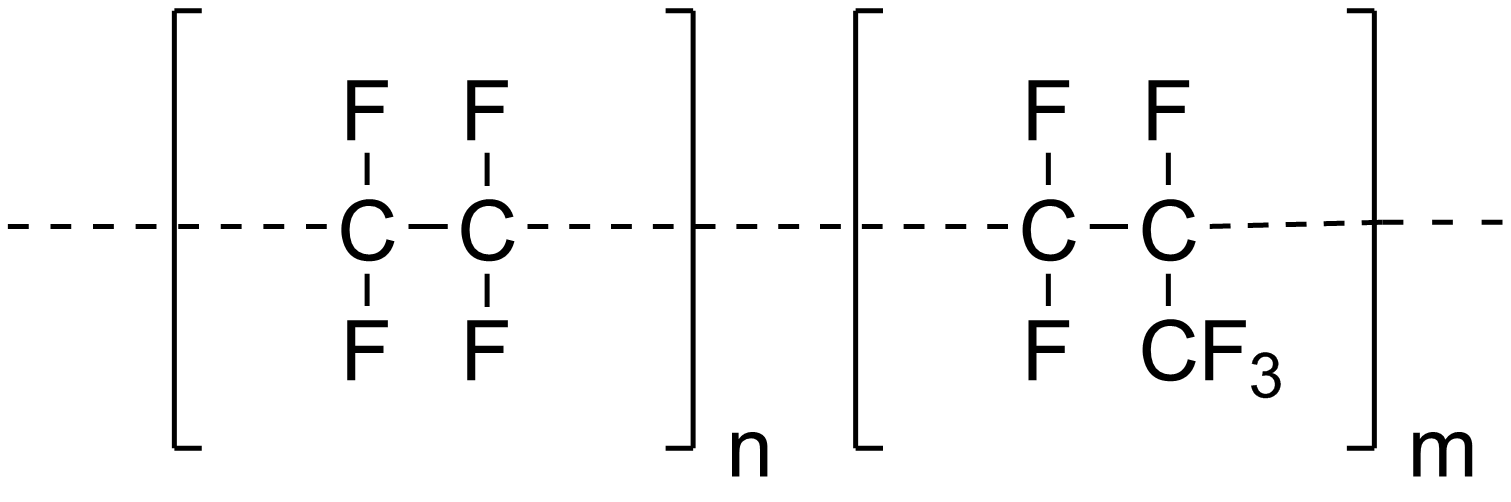
\includegraphics[width=0.5\linewidth]{fig/FEP.png}
    \caption{Molecular Structure of FEP}
    \label{fig:FEP}
\end{figure}

\noindent FEP in the aluminized form was used as the outer layer in the JPL Gen-1 laminate: aluminized Teflon FEP / aluminized Mylar / Vectran / polyurethane \cite{Hall2007_VenusPrototype}. In this configuration FEP provides acid resistance and solar reflectivity (via the aluminium coating), while gas barrier duty is delegated to the aluminized Mylar layer. FEP was later replaced by Aclar (PCTFE) in the Gen-2 laminate due to Aclar's superior toughness and abrasion resistance during handling \cite{Hall2011_TechDev}.



\subsection{Polychlorotrifluoroethylene (PCTFE) - Aclar Film}
\label{ssec:pctfe}


PCTFE (commercially Aclar) is a partially fluorinated polymer with a chlorine substituent on every other carbon along the backbone. It is presented in the Figure \ref{fig:PCTFE}:

\begin{figure}[H]
    \centering
    
\includegraphics[width=0.17\linewidth]{fig/PCTFE.png}
    \caption{Molecular Structure of PCTFE}
    \label{fig:PCTFE}
\end{figure}

\noindent This structural feature results in significantly higher crystallinity than PFA or FEP, which suppresses chain-segment mobility and drastically reduces gas permeability. Among all commercially available fluoropolymers at useful film thicknesses, PCTFE has the lowest gas permeability: N$_2$ permeability is approximately 10\,cm$^3$/m$^2$/d/bar at 25\,µm thickness, comparable to PTFE but in a melt-processible form \cite{PCTFE_Permeability_Guide}. Its H$_2$O vapour permeability is the lowest of any commercial transparent film.

\medskip

\noindent JPL introduced Aclar as the outer film in the Gen-2 Venus balloon laminate precisely because it combines superior gas barrier performance with better abrasion resistance and toughness than FEP \cite{Hall2011_TechDev}. Aclar has a service temperature of approximately 120\,$^\circ$C (limited by the chlorine-containing backbone relative to fully fluorinated alternatives) and acceptable acid resistance at Venus cloud conditions. Its elongation at break is 100-250\%, giving it better flex tolerance than PTFE film \cite{AclarBarrierFilms}.

\medskip

\noindent The primary limitation of PCTFE is that the chlorine atom slightly reduces its chemical inertness relative to pure fluoropolymers: prolonged exposure to very strong reducing agents can break the C-Cl bond. However, at the Venus cloud-level H$_2$SO$_4$ presence (an oxidising rather than reducing acid), this is not considered a failure mode.



\subsection{Biaxially Oriented Polyethylene Terephthalate (BoPET) - Mylar Film}
\label{ssec:mylar}

Mylar (BoPET) is the standard gas-barrier film for terrestrial and planetary balloon applications, shown in the Figure \ref{fig:BoPET}:

\begin{figure}[H]
    \centering
    
\includegraphics[width=0.6\linewidth]{fig/BoPET.png}
    \caption{Molecular Structure of BoPET}
    \label{fig:BoPET}
\end{figure}

Its gas barrier performance in the metallised form (typically 25-75\,nm vacuum-deposited Al layer) approaches that of a continuous metal film for large gas molecules, but metalised Mylar is susceptible to pinhole formation during flexing \cite{MetallizedFilmFlex}. Without metallisation, BoPET has a N$_2$ permeability far too high for multi-year mission. Moreover, which is critical for the given application, the uncoated BoPET is attacked and dissolved by concentrated sulphuric acid \cite{FosterMiller1996_PBOVenus}, which renders it unsuitable for use as an outer layer at Venus. In the Gen-1 JPL laminate, Mylar was retained as an intermediate gas-barrier layer protected from acid contact by the outer FEP layer \cite{Hall2007_VenusPrototype}, which allows to use its benefits while minimising the impact of its weaknesses. 

\medskip

\noindent In the Gen-2 laminate, aluminized Mylar was replaced by thin aluminium foil, which provides a dramatically better helium (and by extension nitrogen) barrier: continuous aluminium foil is impermeable to all gases when free of pinholes, and foil pinholes can be suppressed by lamination tension control and proper seam design \cite{Hall2011_TechDev}. Aluminium foil at 8-12\,µm thickness contributes approximately 20-25\,g/m$^2$ to the laminate areal density, far less than the metallization-plus-Mylar combination for equivalent barrier performance.





\subsection{Vectran Fabric}
\label{ssec:vectran}

Vectran, a liquid-crystal aromatic polyester, poly(hydroxybenzoic acid-co-2-hydroxy-6-naphthoic acid) in the Figure \ref{fig:vectran}, is the structural load-bearing fabric in both JPL Venus balloon prototypes \cite{Hall2007_VenusPrototype,Hall2009_SecondGen}. 

\begin{figure}[H]
    \centering
    
\includegraphics[width=0.5\linewidth]{fig/vectran.png}
    \caption{Molecular Structure of Vectran}
    \label{fig:vectran}
\end{figure}

\noindent As a thermotropic LCP fibre, Vectran's molecular chains are oriented along the fibre axis during melt spinning, giving it tensile strength of approximately 2.9\,GPa and tensile modulus of approximately 70-130\,GPa depending on grade \cite{VectranReview2021}. On a weight-relative basis it is five times stronger than steel \cite{VectranFibrXL}. 

\medskip

\noindent Vectran's thermal performance is well-characterised: it has a melting point of 330\,$^\circ$C and exhibits progressive strength loss above 220\,$^\circ$C, but at the Venus cloud-deck temperature of 35\,$^\circ$C its tensile properties increase slightly relative to ambient temperature. Specifically, its strength increases by approximately +20\% compared to sub-zero temperatures \cite{VectranImattec}. Critically for multi-year superpressure service, Vectran exhibits negligible creep under loads up to 50\% of its breaking strength \cite{VectranFibrXL}, which is the key advantage over para-aramid (Kevlar) fibres in this application.

\medskip

\noindent Vectran is an aromatic polyester; like BoPET, neat Vectran fibre can be attacked by concentrated sulphuric acid if unprotected. In laminate practice, Vectran is always the middle or inner layer, fully encapsulated between the acid-resistant outer film and the inner polyurethane coating, and is therefore never in direct acid contact.

\medskip

\noindent Vectran has a known UV sensitivity, similar to other rigid-rod LCP fibres \cite{VectranImattec}. This is managed in the laminate by the UV-opaque outer fluoropolymer and aluminium layers, which prevent photon access to the Vectran layer.



\subsection{Polybenzoxazole (PBO) - Zylon Film and Fabric}
\label{ssec:pbo}

PBO is a rigid-rod, thermoset liquid-crystalline polymer fibre with the highest tensile strength of any commercially marketed organic fibre at 5.8\,GPa with modulus up to 270\,GPa \cite{ZylonTechnical2005,ZylonSciDirect}. Its limiting oxygen index of 68 and decomposition temperature above 650\,$^\circ$C make it thermally exceptional for Venus applications.

\medskip
\noindent However, PBO has several critical weaknesses for the VISTA concept. First, PBO/Zylon fibres suffer rapid and irrecoverable strength loss under exposure to UV radiation and even visible light \cite{ZylonWiki,ZylonFiberLine}. The mechanism is photodegradation of the benzobisoxazole ring C=N bonds, shown in the Figure \ref{fig:PBO}.


\begin{figure}[H]
    \centering
    
\includegraphics[width=0.5\linewidth]{fig/PBO.png}
    \caption{Molecular Structure of PBO}
    \label{fig:PBO}
\end{figure}

\noindent  At Venus middle cloud level dayside illumination, unprotected PBO would lose more than 50\% of its tensile strength within a period that is short relative to the 5-year mission. Second, technical data confirm that exposure to strong acids causes strength losses and that PBO is more stable than aramid but not immune to H$_2$SO$_4$ \cite{ZylonTechnical2005}. Third, PBO film (as opposed to the PBO fibre) remains at a low TRL for balloon applications. Foster-Miller's PIBO film work was a research-phase activity that never produced a flight-qualified balloon laminate. Fourth, the high modulus of PBO (270\,GPa) goes in parallel with a very low elongation at break (2.5\%) and is effectively brittle in the sense of being flex-fatigue sensitive, with kink-band formation at folded locations being well-documented for all rigid-rod LCP fibres \cite{VectranKinkBand}.

\medskip

\noindent For these reasons, PBO/Zylon is assessed as unsuitable as a structural load-bearing layer for the VISTA dome envelope in the absence of a fully qualified flight demonstration. It may be revisited for future missions targeting lower cloud altitudes where high-temperature capability is the primary driver.


\subsection{Polyurethane (PU) Coating}
\label{ssec:pu}

A thin polyurethane adhesive/sealant coating (Figure \ref{fig:PU}) on the inner surface of the laminate may serve as the bonding layer that binds all outer plies together and provides a thermally sealable inner surface for gore-seam construction. 

\begin{figure}[H]
    \centering
    
\includegraphics[width=0.7\linewidth]{fig/PU.png}
    \caption{Molecular Structure of PU}
    \label{fig:PU}
\end{figure}

In the JPL Gen-1 laminate, PU was the innermost layer \cite{Hall2007_VenusPrototype}. PU has adequate chemical resistance to nitrogen and is compatible with fabric bonding chemistry. It provides elongation and flex tolerance but contributes negligibly to gas barrier performance. Its service temperature of approximately 80-100\,$^\circ$C is adequate for the Venus cloud environment.
\fi




\section{Multi-Layer Laminate Architectures}
\label{sec:mat-architectures}

Given the individual material assessment above, no single film satisfies all material requirements simultaneously. Thus, the design space is multi-layer laminates in which distinct films perform distinct functions. Three architectures are evaluated, reflecting the evolution of JPL Venus balloon technology and VISTA-specific adaptations.


\subsection{Architecture A: JPL Gen-1 Laminate (Baseline Reference)}
\label{ssec:arch-a}

\noindent The first proposed architecture is the laminate flown in the JPL 5.5\,m diameter prototype tested in 2006 \cite{Hall2007_VenusPrototype}. The total areal density is approximately 180\,g/m$^2$. The FEP outer layer provides acid resistance and solar reflectivity via its aluminium coating. The aluminized Mylar provides gas barrier performance. The Vectran fabric provides superpressure burst strength. The polyurethane bonds and seals. This construction achieved a burst superpressure of 39\,200\,Pa and demonstrated 12 days of leak-free hold in Earth testing \cite{Hall2007_VenusPrototype}.

\bigskip

\noindent \textbf{Stack (outside to inside):}
\begin{enumerate}[parsep=0pt]
\item Aluminized FEP film (outer acid barrier and solar reflector)
\item Aluminized Mylar (PET) film (gas barrier)
\item Vectran fabric (structural)
\item Polyurethane adhesive coating
\end{enumerate}

\medskip

\noindent The known weakness of this laminate is the helium permeability of the aluminized Mylar layer: the metalised film develops pinholes during packaging and handling, and helium leaks through these pinholes, limiting float duration to weeks rather than years. This is less critical for VISTA's nitrogen-ISRU architecture because nitrogen molecules are substantially larger and permeate through pinholes more slowly, but the pinhole failure mode is still relevant for structural integrity, especially considering the long mission duration.



\subsection{Architecture B: JPL Gen-2 Laminate with Aluminium Foil}
\label{ssec:arch-b}


\noindent The second-generation JPL Venus balloon laminate was developed after the Gen-1 prototype identified FEP toughness and aluminized Mylar pinhole development as the primary failure drivers \cite{Hall2011_TechDev}. The substitution of Aclar for FEP improves outer-layer toughness and abrasion resistance. The substitution of thin aluminium foil for aluminized Mylar provides a dramatically improved gas barrier because continuous aluminium foil has no inherent polymer permeability channel, only the pinhole population, and pinhole density can be controlled by foil thickness (8-12\,µm) and lamination quality. 

\bigskip
\noindent \textbf{Stack (outside to inside):}
\begin{enumerate}[parsep=0pt]
\item Aclar (PCTFE) film (outer acid barrier)
\item Aluminium foil (gas barrier)
\item Vectran fabric (structural)
\item Polyurethane adhesive coating
\end{enumerate}

\medskip


\noindent For the VISTA nitrogen-ISRU concept, the superior gas retention of the foil layer directly reduces the steady-state nitrogen makeup demand on the ISRU subsystem, which will have a positive waterfall effect on overall performance objectives for such a long-suration mission.

\medskip

\noindent The areal density of this laminate at reference thickness is estimated at 150-170\,g/m$^2$ (depending on Vectran fabric grade and Aclar film thickness). This is at the upper edge of the nominal design case ($\sigma = 150\,\text{g/m}^2$) with a possible slight margin overlap.



\subsection{Architecture C: High-Barrier Thin-Ply Laminate}
\label{ssec:arch-c}

\noindent This architecture replaces the aluminum foil with a second PCTFE film on the inner face of the Vectran fabric, creating a symmetric polymer-only gas barrier that avoids the mechanical fragility of a metallic foil interlayer. The symmetric arrangement ensures that if the outer PCTFE film is locally damaged at a seam, the inner PCTFE film provides a secondary gas barrier. The trade-off is that the gas retention of PCTFE film is lower than that of continuous aluminium foil: PCTFE N$_2$ permeability of approximately 10\,cm$^3$/m$^2$/d/bar at 25\,µm means a measurable steady-state nitrogen flux that must be compensated by the ISRU system. However, for nitrogen (as distinct from helium), the PCTFE N$_2$ retention is expected to be improved given the ISRU replenishment capability.

\bigskip
\noindent
\begin{minipage}[t]{0.42\linewidth}
\textbf{Stack (outside to inside):}
\begin{enumerate}[parsep=0pt]
    \item Aclar (PCTFE) film (outer acid barrier)
    \item Aluminium foil (gas barrier)
    \item Vectran fabric (structural)
    \item Polyurethane adhesive coating
\end{enumerate}
\end{minipage}
\hfill
\begin{minipage}[t]{0.53\linewidth}
For the VISTA nitrogen-ISRU concept, the superior gas retention of the foil layer directly reduces the steady-state nitrogen makeup demand on the ISRU subsystem, which will have a positive waterfall effect on overall performance objectives for such a long-duration mission.
\end{minipage}

\medskip

\noindent The estimated areal density of Architecture C is approximately 140-160\,g/m$^2$, slightly lower than Architecture B if thin PFA (25\,µm) and thin PCTFE (25\,µm each face) films are used. The lower metallic mass fraction also reduces deployed stowed density, which is good for packaging.



\section{Trade-Off Analysis}
\label{sec:mat-tradeoff}

The previous section focused on search of applicable materials and as this task was completed, another stage concerns the choice of the best candidate for the mission at hand. Based on operational conditions outlined in section \ref{sec:mat-environment} and derived requirements from \ref{sec:mat-requirements}, selection criteria can be found and subsequently applied to considered materials.

\subsection{Trade-Off Criteria and Weights}
\label{ssec:tradeoff-criteria}

 The six evaluation criteria are derived directly from the material requirements in Section \ref{sec:mat-requirements}. Weights reflect the mission-critical ranking of each property for the 5-year VISTA float concept.

\begin{table}[H]
\centering
\caption{Trade-off criteria, definitions, and weights for balloon envelope material selection.}
\label{tab:tradeoff-criteria}
\footnotesize
\renewcommand{\arraystretch}{1.15}
\setlength{\tabcolsep}{4pt}
\begin{tabularx}{\linewidth}{@{}p{0.4cm} p{3cm} X p{1.0cm}@{}}
\toprule
\textbf{\#} & \textbf{Criterion} & \textbf{Definition and scoring basis} & \textbf{Weight} \\
\midrule
1 & Acid resistance & Resistance of outer layer to H$_2$SO$_4$ over 5 years; anchored to Venus-specific test data. Score 1 (fails within weeks) to 5 (no degradation, flight-proven). & 25\% \\
2 & Nitrogen gas retention & Estimated total N$_2$ leakage rate per unit area relative to ISRU replenishment capacity; lower leakage = higher score. Score 1 (exceeds ISRU budget) to 5 (minimal leakage, foil-class barrier). & 25\% \\
3 & Specific structural \newline strength & Burst-pressure capacity per unit areal mass; accounts for superpressure structural requirement. Score 1 (insufficient margin) to 5 (substantial margin at $\sigma \leq 150$\,g/m$^2$). & 20\% \\
4 & Flex and deployment tolerance & Ability to survive stowed packaging, deployment shock, and 5-year repeated thermal cycling without pinhole formation or delamination. Score 1 (brittle, pinhole risk) to 5 (no observed degradation in handling tests). & 15\% \\
5 & Long-term UV/thermal stability & Retention of strength and acid resistance under Venus UV irradiance and $\pm$20\,$^\circ$C diurnal cycling for 5 years. Score 1 (rapid photodegradation) to 5 (inherently UV-stable chemistry). & 10\% \\
6 & TRL and flight \newline heritage & Maturity level of the laminate in Venus-relevant testing. Score 1 (concept only) to 5 (flight-tested or full prototype tested at Venus conditions). & 5\% \\
\midrule
\multicolumn{3}{l}{\textit{Total}} & \textbf{100\%} \\
\bottomrule
\end{tabularx}
\end{table}



\subsection{Architecture Scoring}
\label{ssec:tradeoff-scoring}

Upon completing the list of relevant parameters to choose the best-fitting material candidate, a scoring can be assigned to each of considered designs.


\definecolor{score5}{RGB}{0,176,80}
\definecolor{score4}{RGB}{146,208,80}
\definecolor{score3}{RGB}{255,255,0}
\definecolor{score2}{RGB}{255,192,0}
\definecolor{score1}{RGB}{255,0,0}

\begin{table}[H]
\centering
\caption{Scored trade-off matrix for balloon envelope laminate architectures (score 1-5 per criterion; weighted total out of 5).}
\label{tab:tradeoff-matrix}
\footnotesize
\renewcommand{\arraystretch}{1.20}
\setlength{\tabcolsep}{4pt}
\begin{tabularx}{\linewidth}{@{}p{3.3cm}|
>{\centering\arraybackslash}p{1.8cm}|
>{\centering\arraybackslash}p{1.8cm}|
>{\centering\arraybackslash}p{1.6cm}|
>{\centering\arraybackslash}p{1.5cm}|
>{\centering\arraybackslash}p{1.2cm}|
>{\centering\arraybackslash}p{1cm}|
>{\centering\arraybackslash}p{1.3cm}@{}}
\toprule
\textbf{Architecture} &
\textbf{Acid resistance} (25\%) &
\textbf{N$_2$ retention} (25\%) &
\textbf{Sp. strength} (20\%) &
\textbf{Flex tol.} (15\%) &
\textbf{UV/ therm.} (10\%) &
\textbf{TRL} (5\%) &
\textbf{Weighted score} \\
\midrule

\textbf{A} - FEP / Al-Mylar / Vectran / PU &
\cellcolor{score4!40}4 & \cellcolor{score3!40}3 & \cellcolor{score4!40}4 & \cellcolor{score3!40}3 & \cellcolor{score4!40}4 & \cellcolor{score5!40}5 &
\textbf{3.60} \\

\textbf{B} - Aclar / Al-foil / Vectran / PU &
\cellcolor{score5!40}5 & \cellcolor{score5!40}5 & \cellcolor{score4!40}4 & \cellcolor{score4!40}4 & \cellcolor{score5!40}5 & \cellcolor{score4!40}4 &
\textbf{4.55} \\

\textbf{C} - PFA / PCTFE / Vectran / PCTFE / PU &
\cellcolor{score4!40}4 & \cellcolor{score4!40}4 & \cellcolor{score4!40}4 & \cellcolor{score5!40}5 & \cellcolor{score5!40}5 & \cellcolor{score2!40}2 &
\textbf{4.05} \\

\midrule
\multicolumn{8}{@{}p{\linewidth}@{}}{%
\textit{Notes: Scoring rationale is given in Table \ref{tab:scoring-rationale}. The acid resistance score of Architecture B outer (Aclar) is rated 5 based on Hall et al. (2011) sulfuric acid exposure test data showing no degradation of Aclar samples after prolonged immersion testing. Architecture C outer (PFA) is rated 4 because PFA has proven acid resistance at Venus conditions by chemical analogy to FEP, but has less direct Venus balloon-specific test data than Aclar. Architecture C TRL is rated 2 because the symmetric dual-PCTFE inner-face design has not been demonstrated in a Venus balloon prototype.}
} \\
\bottomrule
\end{tabularx}
\end{table}

\noindent As a means of supporting the grading shown in the Table \ref{tab:tradeoff-matrix} above, a list of rationales was compiled in the Table \ref{tab:scoring-rationale} below.

\begin{spacing}{0.95}
\begingroup
\footnotesize
\setlength{\tabcolsep}{2.5pt}
\renewcommand{\arraystretch}{1.12}
\begin{xltabular}{\linewidth}{@{}
>{\RaggedRight\arraybackslash}p{1.6cm}
>{\RaggedRight\arraybackslash}p{1.6cm}
>{\RaggedRight\arraybackslash}X
>{\centering\arraybackslash}p{0.7cm}
@{}}
\caption{Scoring rationale for the balloon envelope material trade-off.}
\label{tab:scoring-rationale} \\
\toprule
\textbf{Arch.} & \textbf{Criterion} & \textbf{Rationale and source basis} & \textbf{Score} \\
\midrule
\endfirsthead
\caption[]{Scoring rationale for the balloon envelope material trade-off. \textit{Continued from previous page.}} \\
\toprule
\textbf{Arch.} & \textbf{Criterion} & \textbf{Rationale and source basis} & \textbf{Score} \\
\midrule
\endhead
\midrule
\multicolumn{4}{r}{\textit{Continued on next page}} \\
\endfoot
\bottomrule
\endlastfoot

A & Acid resist. & FEP outer layer chemically inert to H$_2$SO$_4$ (C-F backbone); flight-proven at VEGA. Minor concern that thin aluminized-FEP surface Al may dissolve locally in prolonged acid, exposing FEP substrate, which is itself robust. Score reduced by 1 from 5 for this minor uncertainty~\cite{Hall2007_VenusPrototype,Kremnev1986}. & 4 \\
A & N$_2$ retention & Aluminized Mylar gas barrier develops pinholes during packaging; direct Gen-1 prototype leakage data showed drift after handling. N$_2$ leakage slower than He by kinetic diameter ratio, partially mitigating, but pinhole mode is non-negligible over 5 years~\cite{Hall2009_SecondGen}. & 3 \\
A & Sp. strength & Vectran fabric layer carries superpressure load; Gen-1 prototype burst at 39\,200\,Pa ($3.3\times$ worst-case)~\cite{Hall2007_VenusPrototype}. Areal density 180\,g/m$^2$ slightly above 150\,g/m$^2$ target. & 4 \\
A & Flex tol. & FEP film is prone to flex cracking relative to Aclar; aluminized Mylar develops pinholes during packaging per Gen-1 testing~\cite{Hall2009_SecondGen}. & 3 \\
A & UV/therm. & FEP inherently UV-stable (C-F); aluminium coating reflects UV from Vectran; all layers thermally stable at 35\,$^\circ$C. CTE mismatch Al/Mylar is manageable~\cite{Hall2007_VenusPrototype}. & 4 \\
A & TRL & Full 5.5\,m prototype fabricated and test-inflated; sulfuric acid coupon tests completed; leakage measured~\cite{Hall2007_VenusPrototype}. & 5 \\
\addlinespace[2pt]
B & Acid resist. & Aclar (PCTFE) outer layer: Hall et al. (2011) report no degradation in sulfuric acid exposure tests; tougher than FEP; no Al surface exposed to acid contact~\cite{Hall2011_TechDev}. & 5 \\
B & N$_2$ retention & Continuous Al foil 8-12\,µm; no intrinsic polymer permeability channel; pinhole density suppressed by lamination quality control; N$_2$ barrier dramatically superior to metallised film~\cite{Hall2011_TechDev}. & 5 \\
B & Sp. strength & Vectran fabric identical to Gen-1; areal density reduced (Aclar + Al foil lighter than FEP + Al-Mylar stack). Estimated 150-165\,g/m$^2$, at the nominal target~\cite{Hall2011_TechDev}. & 4 \\
B & Flex tol. & Aclar (elongation 100-250\%) substantially more flexible than FEP; Al foil brittle at fold lines, but in laminate the Vectran fabric constrains fold geometry; Gen-2 prototype handled without observed delamination~\cite{Hall2011_TechDev,AclarBarrierFilms}. & 4 \\
B & UV/therm. & Aclar inherently UV-stable; Al foil provides additional UV block to Vectran; CTE mismatch Al/polymer over 1825 cycles is a long-term concern not fully tested~\cite{Hall2011_TechDev}. & 5 \\
B & TRL & Aclar/Al-foil/Vectran/PU laminate samples tested in acid and optical tests; aerial deployment tested~\cite{Hall2011_TechDev}. Not full-duration 5-year test; score reduced by 1 from 5. & 4 \\
\addlinespace[2pt]
C & Acid resist. & PFA outer layer: melt-processible, fully fluorinated, proven acid resistance by analogy to PTFE/FEP; less Venus-specific test data than Aclar. Score 4~\cite{FluorocarbonPTFEvsPFA}. & 4 \\
C & N$_2$ retention & Dual PCTFE films (2$\times$25\,µm): combined N$_2$ permeability approximately 5\,cm$^3$/m$^2$/d/bar (doubled thickness halves permeance); no metallic brittleness risk; higher than Al foil but adequate for N$_2$ ISRU budget~\cite{PCTFE_Permeability_Guide}. & 4 \\
C & Sp. strength & Vectran fabric identical; total areal density estimated 140-155\,g/m$^2$; slightly lighter than B, marginally better specific strength. & 4 \\
C & Flex tol. & All-polymer laminate: no brittle metallic interlayer; PFA and PCTFE both have elongation $>$100\%; symmetric structure resists delamination under thermal cycling. No pinholes from flexing expected. Score 5~\cite{AclarBarrierFilms,FEP_PFA_permeability}. & 5 \\
C & UV/therm. & PFA and PCTFE both UV-stable; no CTE mismatch with metallic layer; polymer-only construction expected to have excellent thermal cycling fatigue life. Score 5. & 5 \\
C & TRL & Symmetric dual-PCTFE architecture not demonstrated in any Venus balloon prototype; concept only. Score 2~\cite{Hall2011_TechDev}. & 2 \\
\end{xltabular}
\endgroup
\end{spacing}


\section{Selected Architecture and Design Specification}
\label{sec:mat-selection}

Architecture B (Aclar PCTFE / Aluminium foil / Vectran fabric / Polyurethane coating, from outside to inside) is selected as the baseline VISTA balloon envelope material. It achieves the highest weighted score of 4.55/5.00, excelling on the two highest-weighted criteria (acid resistance and nitrogen gas retention). The selection is reinforced by the highest available TRL: the Aclar/Al-foil/Vectran/PU laminate has been fabricated, acid-tested, optically characterised, and aerially deployed by the JPL team \cite{Hall2011_TechDev}, making it the most mature Venus-specific balloon laminate in the open literature.

\subsection{Selection Specification}


The selected laminate specification is given in Table \ref{tab:laminate-spec}. Layer thicknesses reflect the Gen-2 prototype design reported by Hall et al. \cite{Hall2011_TechDev}, with the Vectran grade selected to match the superpressure structural requirement.

\begin{table}[H]
\centering
\caption{Selected VISTA balloon envelope laminate specification (Architecture B).}
\label{tab:laminate-spec}
\footnotesize
\renewcommand{\arraystretch}{1.18}
\setlength{\tabcolsep}{4pt}
\begin{tabularx}{\linewidth}{@{}
>{\centering\arraybackslash}p{0.5cm}
p{4cm}
p{4cm}
p{2.2cm}
p{1.5cm}
X
@{}}
\toprule
\textbf{Ply} & \textbf{Material} & \textbf{Function} & \textbf{Thick.} & \textbf{Areal mass} & \textbf{Key references} \\
\midrule
1 (out.) & Aclar PCTFE film & Acid barrier, abrasion resistance & 25\,µm & $\approx$38\,g/m$^2$ & \cite{Hall2011_TechDev,PCTFE_Permeability_Guide} \\
2 & Aluminium foil (hard-rolled) & Gas barrier (N$_2$/He) & 10\,µm & $\approx$27\,g/m$^2$ & \cite{Hall2011_TechDev} \\
3 & Vectran HS fabric, 2$\times$2 twill & Superpressure structural layer & $\approx$180\,µm & $\approx$75\,g/m$^2$ & \cite{Hall2007_VenusPrototype,VectranReview2021} \\
4 (inn.) & Polyurethane adhesive/seal coat & Bonding, seaming, inner seal & 15\,µm & $\approx$15\,g/m$^2$ & \cite{Hall2007_VenusPrototype} \\
\midrule
\multicolumn{3}{l}{\textbf{Total laminate}} & $\approx$230\,µm & $\approx$155\,g/m$^2$ & Within nominal ROM $\sigma$ case. \\
\bottomrule
\end{tabularx}
\end{table}

\noindent The total areal density of approximately 155\,g/m$^2$ is consistent with the nominal ROM envelope sizing at $\sigma = 150\,\text{g/m}^2$, with the 5\,g/m$^2$ difference within the 20\% early-phase mass margin already applied in the buoyancy calculation. The seam construction follows the bi-taped gore-seam approach of the JPL prototypes, using a sulphuric-acid-resistant adhesive on the exposed outer seam surfaces \cite{Hall2007_VenusPrototype}.



\subsection{Compliance with Material Requirements}
\label{ssec:mat-compliance}

Finally, the chosen material can be formally confronted with predefined subsystem requirements from section \ref{sec:mat-requirements}, the effect of which is shown in the Table \ref{tab:mat-compliance} below.

\begin{table}[H]
\centering
\caption{Compliance assessment of the selected laminate against material-level requirements.}
\label{tab:mat-compliance}
\footnotesize
\renewcommand{\arraystretch}{1.15}
\setlength{\tabcolsep}{4pt}
\begin{tabularx}{\linewidth}{@{}p{2.0cm} X p{1.2cm}@{}}
\toprule
\textbf{Requirement} & \textbf{Compliance evidence} & \textbf{Status} \\
\midrule
REQ-MAT-01 (acid) & Aclar outer ply: Hall et al. (2011) sulfuric acid coupon tests show no degradation; PCTFE chemistry fully inert to H$_2$SO$_4$ at 35\,$^\circ$C. & \checkmark \\
REQ-MAT-02 (N$_2$ retention) & Al foil gas barrier: continuous foil has near-zero polymer permeance; N$_2$ loss via pinholes manageable by ISRU at 15\,W steady state. & \checkmark \\
REQ-MAT-03 (tensile) & Vectran HS fabric: Gen-1 prototype burst at $3.3\times$ worst-case superpressure~\cite{Hall2007_VenusPrototype}. Safety factor $\geq$3 met. & \checkmark \\
REQ-MAT-04 (areal mass) & $\approx$155\,g/m$^2$ estimated; within 20\% mass margin of $\sigma = 150\,\text{g/m}^2$ nominal. & \checkmark \\
REQ-MAT-05 (flex) & Aclar elongation 100-250\%~\cite{AclarBarrierFilms}; Vectran fabric constrains foil fold geometry; no pinhole formation reported in Gen-2 handling tests~\cite{Hall2011_TechDev}. & \checkmark \\
REQ-MAT-06 (UV/therm.) & PCTFE and Al UV-opaque and stable; Vectran UV-sensitive but fully encapsulated; all layers thermally rated for 35\,$^\circ$C service. & \checkmark \\
REQ-MAT-07 (TRL) & Aclar/Al-foil/Vectran/PU samples: Venus acid-testing and aerial deployment completed by JPL~\cite{Hall2011_TechDev}. TRL assessed at 4-5. & \checkmark \\
\bottomrule
\end{tabularx}
\end{table}



\subsection{Residual Risks}
\label{ssec:mat-risks}

Three residual risks are identified for this material selection at the current design phase.

\begin{enumerate}
    \item \textbf{Risk 1} - Long-term CTE fatigue \\The aluminium foil (CTE $\approx$23\,ppm/K) and PCTFE film (CTE $\approx$70\,ppm/K) have a CTE mismatch of approximately 47\,ppm/K. Over 1825 diurnal cycles in thermal cycling, the accumulated shear strain at the foil-film interface will have a non-negligible impact. This is managed by the Vectran fabric, which mechanically constrains deformation, but delamination propagation from a seam edge still needs to be assessed. 
    \item \textbf{Risk 2} - Seam acid ingress \\The outer seam uses an acid-resistant adhesive, but the tape edges represent a potential ingress path for H$_2$SO$_4$ to reach aluminium foil, which is not acid-resistant. Foil corrosion would open a local gas-barrier breach. The mitigation is to lap the Aclar outer-ply edge fully over the tape \cite{Hall2011_TechDev}.
    \item \textbf{Risk 3} - Pinhole population in foil\\ Idealized pure-lattice aluminium foil has an extremely low permeability but - depending on manufacturing quality and handling - a finite pinhole population. The Gen-2 test programme at JPL did not measure the impact of these impurities quantitatively and thus a full characterisation test campaign is required before the final N$_2$ leakage rate can be confirmed.
\end{enumerate}

\noindent These shall be addressed in following design stages, as well as the planned tests to reliably confirm set assumptions and verify the stated TRL.


\section{Balloon Sizing}

\subsection*{ISRU and Balloon Architecture}

\begin{figure}[H]
    \centering
    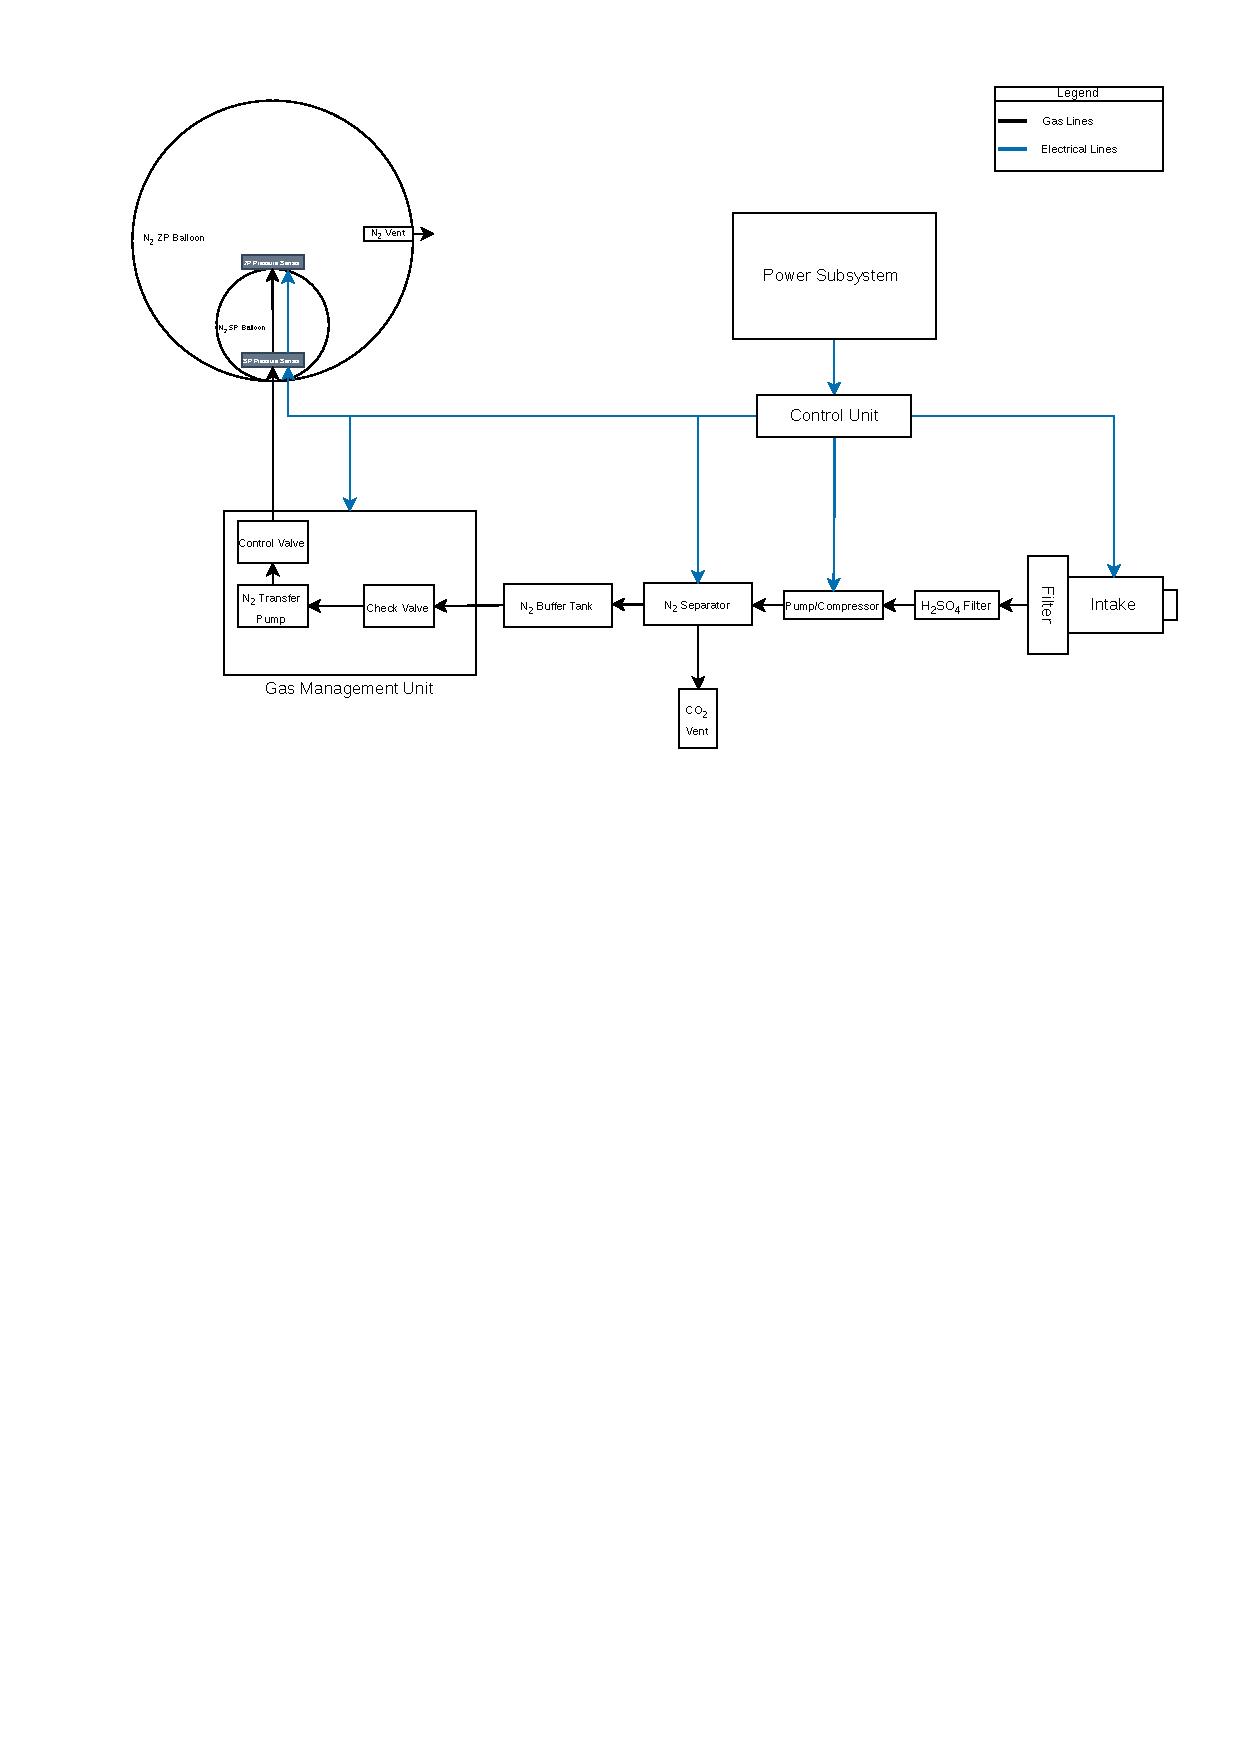
\includegraphics[draft=false,width=0.7\textwidth]{fig/ISRU_arch.pdf}
    \caption{ISRU and Balloon System}
    \label{ISRU_architecture}
\end{figure}



\begin{table}[H]
\centering
\caption{Material properties used for the balloon envelope sizing.}
\label{tab:balloon_material_properties}
\renewcommand{\arraystretch}{1.25}
\setlength{\tabcolsep}{6pt}
\begin{tabular}{l l c c c}
\hline
\textbf{Material layer} & \textbf{Main role} & 
\textbf{Thickness} & 
\textbf{Areal density} & 
\textbf{$N_2$ permeability} \\
& & 
\textbf{[$\mu$m]} & 
\textbf{[g/m$^2$]} & 
\textbf{[Barrer]} \\
\hline
Aclar PCTFE & Acid / gas barrier & 25 & 38 & 0.188~\cite{Kianfar2021} \\
Aluminium foil & Gas barrier & 10 & 27 & 0.5 \\
Vectran HS & Structural layer & 180 & 75 & $1.0 \times 10^{6}$ \\
Polyurethane (PU) & Seal / gas barrier layer & 15 & 15 & 3.25~\cite{Semsarzadeh2008PU} \\
\hline
Outer ZP envelope & Aclar + Al + PU & 50 & 80 & 0.317 \\
Inner SP envelope & Vectran HS + PU + Al & 205 & 117 & 8.328 \\ 
\hline
\end{tabular}
\end{table}

\begin{flushleft}
\footnotesize
$^{*}$ Effective permeability calculated using the series-resistance approximation \cite{Vercasson2025}:
\begin{align*}
P_{\mathrm{eff}} =
\frac{t_{\mathrm{tot}}}
{\sum_i \frac{t_i}{P_i}}
\end{align*}
where $t_i$ and $P_i$ are the thickness and nitrogen permeability of each layer.
The Vectran permeability is set to a very large value in the model, meaning that it is treated as a structural layer rather than a gas-barrier layer. The permeability value for Aluminum foil is assumed to be 0.5 \cite{Stanford1963N2O4}, in order to account for pinholes, connections and potential defects. It is a conservative, defect-adjusted effective permeability for the aluminum foil layer.
\end{flushleft}


The constants used in the code for balloon sizing are also listed in the following table:

\begin{table}[H]
\centering
\caption{Constants used in the balloon sizing model}
\label{tab:balloon_sizing_constants}
\renewcommand{\arraystretch}{1}
\begin{tabular}{l l l}
\hline
\textbf{Symbol / variable} & \textbf{Definition} & \textbf{Value} \\
\hline
$x_{N_2,\mathrm{Venus}}$ & Venus atmospheric nitrogen mole fraction & $0.035$ \\
$M_{N_2}$ & Molar mass of nitrogen & $0.0280134~\mathrm{kg/mol}$ \\
$g_{\mathrm{Venus}}$ & Venus gravitational acceleration & $8.87~\mathrm{m/s^2}$ \\
$C_D$ & Balloon drag coefficient & $0.5$ \\
$M_{\mathrm{carry}}$ & Gondola, payload, and support mass & $94~\mathrm{kg}$ \\
$\Delta p_{\mathrm{SP}}$ & Superpressure differential & $25000~\mathrm{Pa}$ \\
$D_{\mathrm{SP}}/D_{\mathrm{outer}}$ & SP-to-outer balloon diameter ratio & $0.5$ \\
$B_{\mathrm{SI}}$ & Barrer-to-SI conversion factor & $3.348\times10^{-16}~\mathrm{mol\,m/(m^2\,s\,Pa)}$ \\
$\mathrm{margin}_{\mathrm{env}}$ & Envelope mass margin & $0.15$ \\
$FS_{\mathrm{SP}}$ & Superpressure balloon factor of safety & $2.0$ \\
$\sigma_{\mathrm{Vectran,ult}}$ & Vectran ultimate tensile strength & $3\times10^9~\mathrm{Pa}$ \\
$k_{\mathrm{crimp}}$ & Crimp knockdown factor & $0.80$ \cite{Hall2021}\\
$k_{\mathrm{biaxial}}$ & Biaxial loading knockdown factor & $0.77$ \\
$k_{\mathrm{seam}}$ & Seam knockdown factor & $0.80$ \\
$k_{\mathrm{thermal}}$ & Thermal knockdown factor & $0.75$ \\
\hline
\end{tabular}
\end{table}

\subsection*{Main Assumptions}
This sizing model is preliminary, hence several assumptions are made to simplify the initial sizing approach:

\begin{enumerate}
    \item The balloon is assumed to be spherical. In reality, the balloon will have changes in curvature, seams, local wrinkling, and non-spherical deformation.
    \item The gas is assumed to behave ideally. Therefore, the gas density is calculated using the ideal gas law:
    \begin{align}
        \rho = \frac{pM}{RT}
    \end{align}
    where $\rho$ is the gas density, $p$ is the pressure, $M$ is the molar mass, $R$ is the universal gas constant, and $T$ is the temperature.
    \item The superpressure-to-zero-pressure diameter ratio is fixed at:
    \begin{align}
        \frac{D_{\mathrm{SP}}}{D_{\mathrm{ZP}}} = 0.5
    \end{align}
    This follows the preliminary balloon-in-balloon sizing assumption based on Hall et al.~\cite{Hall2021}. Since volume scales with diameter cubed, this gives:
    \begin{align}
        \frac{V_{\mathrm{SP}}}{V_{\mathrm{ZP}}} =
        \left(\frac{D_{\mathrm{SP}}}{D_{\mathrm{ZP}}}\right)^3
        = 0.5^3 = 0.125
    \end{align}
    \item The superpressure differential is fixed at:
    \begin{align}
        \Delta p_{\mathrm{SP}} = 25{,}000~\mathrm{Pa}
    \end{align}
    This is used as a representative preliminary superpressure value based on Hall et al.~\cite{Hall2021}.
\end{enumerate}
\subsection{Sizing Procedure}

The process of sizing the balloon was based on the equilibrium sizing procedure presented by Hall et al.~\cite{Hall2021}, originally developed for helium, and adapted here for nitrogen. Since the balloon is intended to operate in the Venus cloud/habitable zone, the altitude range and corresponding atmospheric properties were first defined. The model considers altitudes from $52$ to $62~\mathrm{km}$, with atmospheric temperature, pressure, and density specified at each altitude.

% Paste atmospheric data table from the code here.

Following Hall et al.~\cite{Hall2021}, a worst-case sustained vertical wind speed of 
$3~\mathrm{m/s}$ is considered for preliminary Venus aerobot sizing. The corresponding drag force is

\begin{equation}
    F_{\mathrm{drag}}
    =
    \frac{1}{2}
    \rho_{\mathrm{atm}}
    S_{\mathrm{ref}}
    v_{\mathrm{wind}}^2
    C_D ,
\end{equation}

where $\rho_{\mathrm{atm}}$, $S_{\mathrm{ref}}$, $v_{\mathrm{wind}}$ and $C_D$ are the atmospheric density, projected balloon area, vertical wind speed and drag coefficient, respectively. In the model, this is converted into an equivalent mass penalty:

\begin{equation}
    m_{\mathrm{drag}}
    =
    \frac{F_{\mathrm{drag}}}{g_{\mathrm{Venus}}}
    =
    \frac{
    \rho_{\mathrm{atm}}S_{\mathrm{ref}}v_{\mathrm{wind}}^2C_D
    }
    {2g_{\mathrm{Venus}}}.
\end{equation}
A static force balance is used to find the required outer balloon volume. The displaced atmospheric mass must balance the carried mass, envelope mass, nitrogen mass and vertical-wind drag penalty:
\begin{equation}
    \rho_{\mathrm{atm}}V_{\mathrm{outer}}
    =
    M_{\mathrm{carry}}
    +
    m_{\mathrm{env,total}}
    +
    \rho_{N_2}V_{\mathrm{ZP}}
    +
    \rho_{N_2,\mathrm{SP}}V_{\mathrm{SP}}
    +
    m_{\mathrm{drag}} .
\end{equation}
Here, $M_{\mathrm{carry}}$ is the gondola, payload and support mass, taken as $94~\mathrm{kg}$. Since the envelope and drag areas depend on the balloon volume, the equation is solved numerically for $V_{\mathrm{outer}}$ using bisection.

The SP volume is calculated from the assumed diameter ratio:
\begin{equation}
    V_{\mathrm{SP}}
    =
    \left(\frac{D_{\mathrm{SP}}}{D_{\mathrm{outer}}}\right)^3
    V_{\mathrm{outer}},
\end{equation}
and the ZP gas volume is then
\begin{equation}
    V_{\mathrm{ZP}}
    =
    V_{\mathrm{outer}} - V_{\mathrm{SP}} .
\end{equation}

Assuming spherical envelopes, the surface areas are calculated from the corresponding diameters. Using the areal densities from \autoref{tab:balloon_material_properties}, the total envelope mass is
\begin{equation}
    m_{\mathrm{env,total}}
    =
    w_{\mathrm{outer}}A_{\mathrm{outer}}
    +
    w_{\mathrm{SP}}A_{\mathrm{SP}} .
\end{equation}

The nitrogen densities are calculated using the ideal gas law. The ZP balloon is assumed to be at ambient pressure, while the SP balloon is pressurised by the imposed superpressure differential:
\begin{align}
    \rho_{N_2}
    &=
    \frac{pM_{N_2}}{RT},
    &
    \rho_{N_2,\mathrm{SP}}
    &=
    \frac{(p+\Delta p_{\mathrm{SP}})M_{N_2}}{RT}.
\end{align}
The nitrogen mass is split between the ZP and SP volumes, giving:
\begin{equation}
    m_{N_2,\mathrm{total}}
    =
    \rho_{N_2}V_{\mathrm{ZP}}
    +
    \rho_{N_2,\mathrm{SP}}V_{\mathrm{SP}} .
\end{equation}
The outer and inner envelope equivalent thicknesses are calculated from the areal density and equivalent material density:
\begin{align}
    t =
    \frac{w}{\rho_{\mathrm{mat}}}
\end{align}
Since the superpressure balloon is pressurised, its envelope experiences membrane stress. For a thin spherical pressure vessel, the membrane stress is calculated as:
\begin{align}
    \sigma_{\mathrm{SP}} =
    \frac{\Delta p_{\mathrm{SP}} r_{\mathrm{SP}}}
    {2t_{\mathrm{SP}}}
\end{align}
where $\sigma_{\mathrm{SP}}$ is the SP membrane stress, $\Delta p_{\mathrm{SP}}$ is the superpressure differential, $r_{\mathrm{SP}}$ is the SP balloon radius, and $t_{\mathrm{SP}}$ is the SP envelope thickness.

The leakage rate is estimated using a steady-state permeation model:
\begin{equation}
    \dot{n}_{N_2}
    =
    \frac{P_{\mathrm{eff}}A\Delta p_{N_2}}{t},
\end{equation}
where $P_{\mathrm{eff}}$, $A$, $\Delta p_{N_2}$ and $t$ are the effective permeability, envelope area, nitrogen partial-pressure difference and envelope thickness, respectively. For the outer envelope, the nitrogen partial-pressure difference is approximated as
\begin{equation}
    \Delta p_{N_2,\mathrm{outer}}
    =
    p(1-x_{N_2,\mathrm{Venus}}).
\end{equation}
The nitrogen replenishment rate is assumed equal to the external leakage through the outer envelope, which is converted to kg/day using
\begin{equation}
    \dot{m}_{N_2,\mathrm{day}}
    =
    \dot{n}_{N_2}M_{N_2}\cdot86400 .
\end{equation}
This calculation is repeated for each altitude and vertical wind-speed case.

A worst-case SP structural check is then performed over all altitude and wind-speed cases. Since membrane stress increases with radius, the largest SP radius is used to calculate the stress-required thickness:
\begin{equation}
    t_{\mathrm{SP,stress}}
    =
    \frac{\Delta p_{\mathrm{SP}}r_{\mathrm{SP,max}}}
    {2\sigma_{\mathrm{allow,SP}}}.
\end{equation}
The allowable SP stress is calculated using knockdown factors and a safety factor, following the approach in Hall et al.~\cite{Hall2021}:
\begin{equation}
    \sigma_{\mathrm{allow,SP}}
    =
    \frac{
    \sigma_{\mathrm{Vectran,ult}}
    k_{\mathrm{crimp}}
    k_{\mathrm{biaxial}}
    k_{\mathrm{seam}}
    k_{\mathrm{thermal}}
    }
    {FS_{\mathrm{SP}}}.
\end{equation}
The final SP design thickness is taken as
\begin{equation}
    t_{\mathrm{SP,design}}
    =
    \max\left(t_{\mathrm{SP,material}},t_{\mathrm{SP,stress}}\right).
\end{equation}
If the stress-required thickness exceeds the selected material thickness, the SP areal density is updated and the altitude/wind-speed sweep is repeated, since the increased envelope mass affects the required volume and all dependent outputs.

The results are visualised in the following plots:

% Paste the plots here.

\begin{figure}[H]
    \centering

    \begin{subfigure}{0.42\textwidth}
        \centering
        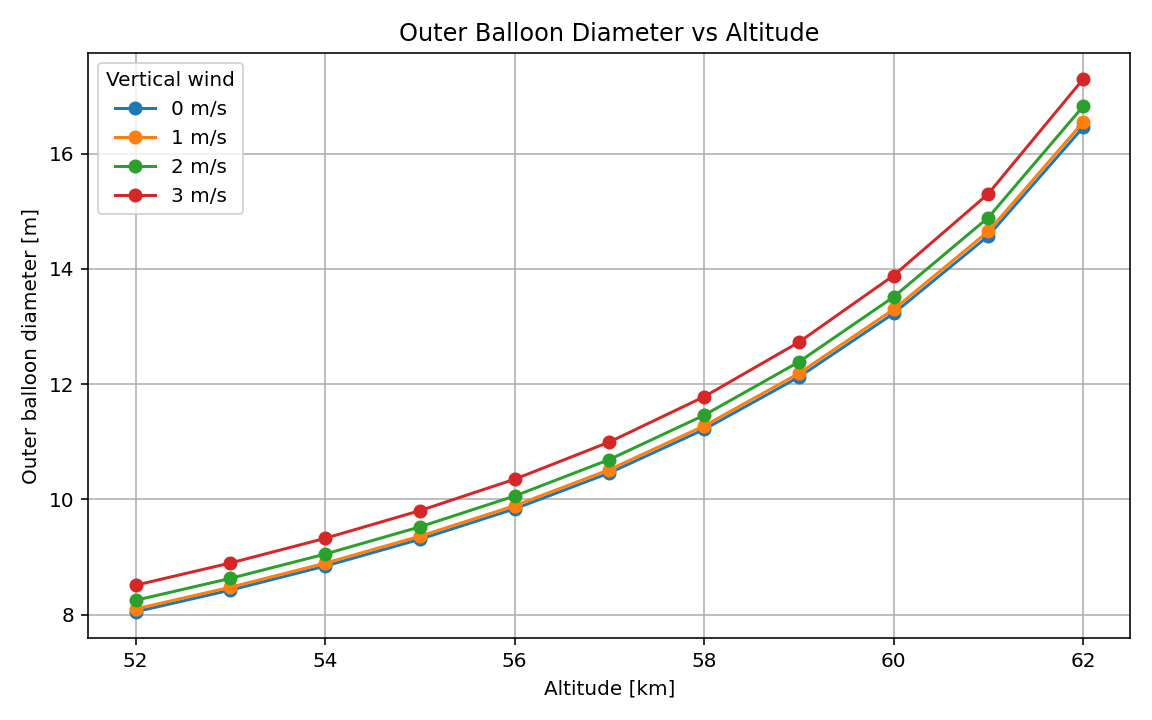
\includegraphics[width=\textwidth]{fig/Diam_plot.png}
        \caption{Outer diameter vs altitude}
        \label{fig:diameter_altitude}
    \end{subfigure}
    \hspace{0.04\textwidth}
    \begin{subfigure}{0.42\textwidth}
        \centering
        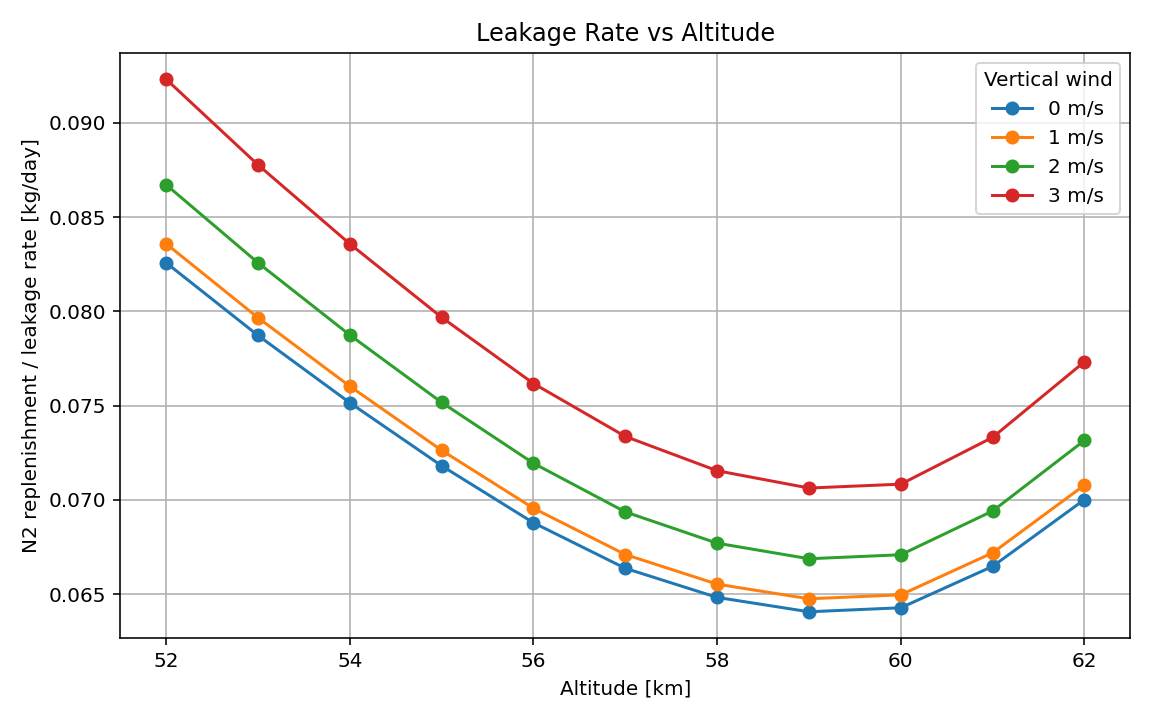
\includegraphics[width=\textwidth]{fig/Leakage_plot.png}
        \caption{N$_2$ leakage rate vs altitude}
        \label{fig:leakage_altitude}
    \end{subfigure}

    \caption{Balloon diameter and nitrogen leakage rate as a function of altitude for different vertical wind speeds.}
    \label{fig:balloon_sizing_results}
\end{figure}

Finally, the dry envelope mass of the selected configuration is calculated from the design surface areas and corresponding areal densities. A 15\% mass margin is then applied:
\begin{equation}
    m_{\mathrm{env,total,margin}}
    =
    \left(
    w_{\mathrm{outer}}A_{\mathrm{outer,design}}
    +
    w_{\mathrm{SP}}A_{\mathrm{SP,design}}
    \right)
    (1+\mathrm{margin}) .
\end{equation}
The results are summarised in the tables below. The leakage values include the applied factor-of-two sizing margin and are taken over the full altitude and vertical wind-speed sweep.

% Paste the results summary table here.

\begin{table}[H]
\centering
\caption{Envelope mass, nitrogen mass, and leakage results}
\label{tab:mass_and_leakage_results}
\renewcommand{\arraystretch}{1.08}
\small

\begin{minipage}{0.56\textwidth}
\centering
\begin{tabular}{cc@{\quad}cc}
\toprule
\multicolumn{2}{c}{\textbf{Envelope}} &
\multicolumn{2}{c}{\textbf{N$_2$ at 55 km}} \\
\cmidrule(lr){1-2} \cmidrule(lr){3-4}
$h_{\max}$ [km] & $m_{\mathrm{env}}$ [kg] &
$v_{\mathrm{wind}}$ [m/s] & $m_{N_2}$ [kg] \\
\midrule
60 & 83.83  & 0 & 264.89 \\
62 & 118.03 & 1 & 269.45 \\
   &        & 2 & 283.70 \\
   &        & 3 & 309.61 \\
\bottomrule
\end{tabular}
\end{minipage}
\hfill
\begin{minipage}{0.38\textwidth}
\centering
\begin{tabular}{lc}
\toprule
\multicolumn{2}{c}{\textbf{N$_2$ Leakage}} \\
\cmidrule(lr){1-2}
\textbf{Case} & \textbf{$\dot{m}_{N_2}$ [kg/day]} \\
\midrule
Average over sweep & 0.146 \\
Maximum over sweep & 0.185 \\
\bottomrule
\end{tabular}
\end{minipage}

\end{table}

For the rest of this report, a conservative value of 0.185 kg for the N2 flow rate will be used. It represents a maximum replenishment rate over the entire altitude-wind sweep, with a safety margin of 2.0. This margin makes sense, since the values for N2 leakage are based on an ideal membrane permeation model, and therefore do not account for manufacturing defects, degradation, pinholes etc. 





\section{ISRU Power Consumption Estimation}

As can be seen in \autoref{ISRU_architecture}, the ISRU system contains several components that consume electrical power. Some of the known values used in the power estimation are defined in Table~\ref{tab:isru_power_inputs}.

\begin{table}[H]
\centering
\caption{Fixed input values used in the ISRU power estimation}
\label{tab:isru_power_inputs}
\renewcommand{\arraystretch}{1}
\begin{tabular}{l l c}
\toprule
\textbf{Variable} & \textbf{Description} & \textbf{Value} \\
\midrule
$T_0$ & Reference separation temperature & $300~\mathrm{K}$ \cite{Hall2021} \\
$E_{\mathrm{PSA,air}}$ & PSA nitrogen specific energy for Earth air & $0.63~\mathrm{kWh/kg_{N_2}}$ \\
$x_{N_2,\mathrm{air}}$ & Nitrogen mole fraction in Earth air & $0.7808$ \\
$\gamma_{N_2}$ & Nitrogen specific heat ratio & $1.4$ \\
$\eta_{\mathrm{comp}}$ & Compressor efficiency & $0.50$ \\
$T_{\mathrm{ref}}$ & Reference compressor inlet temperature & $302.3~\mathrm{K}$ \cite{Hall2021} \\
$p_{\mathrm{ref}}$ & Reference atmospheric pressure at 55 km & $53183~\mathrm{Pa}$ \cite{Hall2021} \\
$\Delta p_{\mathrm{SP}}$ & Superpressure differential & $25000~\mathrm{Pa}$ \\
$\dot{m}_{N_2,\mathrm{transfer}}$ & Daily N$_2$ transfer between ZP and SP balloons & $15~\mathrm{kg/day}$ \\
$P_{\mathrm{valve}}$ & Rated valve power & $7.8~\mathrm{W}$ \\
$DC_{\mathrm{valve}}$ & Valve duty cycle & $0.05$ \\
$P_{\mathrm{control}}$ & Control unit power & $0.4~\mathrm{W}$ \\
$P_{\mathrm{sensor}}$ & Pressure sensor power & $0.5~\mathrm{W}$ \\
$P_{\mathrm{intake,rated}}$ & Rated intake pump power & $12 ~\mathrm{W}$ \\
$DC_{\mathrm{intake}}$ & Intake pump duty cycle & $0.5$ \\
\bottomrule
\end{tabular}
\end{table}

Values for the intake pump, nitrogen separator, and nitrogen pump for altitude control need to be calculated based on the required nitrogen replenishment rate, defined previously in Table~\ref{tab:n2_leakage_summary}. Firstly, as stated in \autoref{sec:n2_separation_tradeoff}, at this stage a PSA system is used for separating N$_2$ from CO$_2$. On Earth, the nitrogen separation energy is based on a PSA specific energy of $0.63~\mathrm{kWh/kg_{N_2}}$ \cite{Rinker2024}, which is used as a conservative baseline value. However, since the N$_2$ concentration in the Venus atmosphere is only $3.5\%$, compared to approximately $78\%$ on Earth, a correction factor is needed. For this, the ideal minimum Gibbs work of separation is used. The minimum separation work per mole of nitrogen product is calculated as \cite{Ghoniem2020}:
\begin{align}
    w_{\min}(x) =
    -RT_0
    \left[
    \ln(x)
    +
    \frac{1-x}{x}\ln(1-x)
    \right]
\end{align}
The correction factor is then defined as:
\begin{align}
    f_{\mathrm{thermal}} =
    \frac{
    w_{\min}(x_{N_2,\mathrm{Venus}})
    }
    {
    w_{\min}(x_{N_2,\mathrm{air}})
    }
\end{align}
The Venus-adjusted ISRU specific energy is therefore:
\begin{align}
    E_{\mathrm{ISRU}} =
    E_{\mathrm{PSA,air}} f_{\mathrm{thermal}}
\end{align}
The average gas-processing power of the separator is then calculated from the daily nitrogen replenishment rate as:
\begin{align}
    P_{\mathrm{gas}} =
    \frac{
    \dot{m}_{N_2,\mathrm{repl}} E_{\mathrm{ISRU}}
    }
    {24}
    \cdot 1000
\end{align}
where $\dot{m}_{N_2,\mathrm{repl}}$ is the nitrogen replenishment rate in $\mathrm{kg/day}$, $E_{\mathrm{ISRU}}$ is the Venus-adjusted specific energy in $\mathrm{kWh/kg}$, and the factor of $1000$ converts the result from kW to W.

In order to calculate the power consumption of the N$_2$ pump, which pumps nitrogen between the SP and ZP balloons and is used for altitude control, the compressor power is calculated using the standard compressor relation. First, the pressure ratio is defined as:
\begin{align}
    \Pi_c =
    \frac{P_{\mathrm{out}}}{P_{\mathrm{in}}}
    =
    \frac{p_{\mathrm{ref}}+\Delta p_{\mathrm{SP}}}
    {p_{\mathrm{ref}}}
\end{align}
where $P_{\mathrm{in}}$ is the inlet pressure and $P_{\mathrm{out}}$ is the outlet pressure. The nitrogen-specific gas constant is:
\begin{align}
    R_{\mathrm{spec},N_2} =
    \frac{R}{M_{N_2}}
\end{align}
The specific heat at constant pressure is then estimated as:
\begin{align}
    c_{p,N_2} =
    \frac{\gamma_{N_2}}{\gamma_{N_2}-1}
    R_{\mathrm{spec},N_2}
\end{align}
The compressor work per kilogram of nitrogen is estimated using \cite{NASAGlennCompressor}:
\begin{align}
    w_{\mathrm{comp}} =
    \frac{
    c_{p,N_2} T_{\mathrm{ref}}
    \left[
    \Pi_c^{\frac{\gamma_{N_2}-1}{\gamma_{N_2}}}
    -1
    \right]
    }
    {\eta_{\mathrm{comp}}}
\end{align}
where $w_{\mathrm{comp}}$ is the compressor work per kilogram, $c_{p,N_2}$ is the specific heat at constant pressure, $T_{\mathrm{ref}}$ is the reference inlet temperature, $\Pi_c$ is the pressure ratio, and $\eta_{\mathrm{comp}}$ is the compressor efficiency.

The compressor energy is converted from $\mathrm{J/kg}$ to $\mathrm{kWh/kg}$ using:
\begin{align}
    E_{\mathrm{altitude}} =
    \frac{w_{\mathrm{comp}}}{3.6\times10^6}
\end{align}
The average altitude-control power is therefore:
\begin{align}
    P_{\mathrm{altitude}} =
    \frac{
    \dot{m}_{N_2,\mathrm{transfer}}
    E_{\mathrm{altitude}}
    }
    {24}
    \cdot 1000
\end{align}
where $\dot{m}_{N_2,\mathrm{transfer}}$ is defined as $15~\mathrm{kg/day}$, which is the assumed average amount of nitrogen pumped between the SP and ZP balloons per day.

The auxiliary power includes the valves, controller, intake compressor, and two pressure sensors, located in the superpressure balloon and one inside the zero-pressure balloon, with the values defined in Table~\ref{tab:isru_power_inputs}. Finally, the total ISRU power consumption can be computed from adding all components:
\begin{align}
    P_{\mathrm{aux}} &=
    P_{\mathrm{valves}}
    +
    P_{\mathrm{control}}
    +
    P_{\mathrm{sensors}}
    \\
    P_{\mathrm{gas,final}} &=
    P_{\mathrm{gas}}
    +
    P_{\mathrm{intake}}
    \\
    P_{\mathrm{ISRU,total}} &=
    P_{\mathrm{aux}}
    +
    P_{\mathrm{gas,final}}
    +
    P_{\mathrm{altitude}}
\end{align}
The final results can be found in the table below:

% Paste final ISRU power results table here.

\begin{table}[H]
\centering
\caption{ISRU power consumption for average and maximum replenishment cases}
\label{tab:isru_power_results}
\renewcommand{\arraystretch}{1.15}
\small
\begin{tabular}{p{4.2cm} c c}
\toprule
\textbf{Case} & 
\textbf{$\dot{m}_{N_2}$ [kg/day]} & 
\textbf{$P$ [W]} \\
\midrule
Average replenishment, SF = 2.0 
& 0.146 & 45.498 \\

Maximum replenishment, SF = 2.0 
& 0.185 & 52.448 \\
\bottomrule
\end{tabular}
\end{table}

\section{Sensitivity Analysis}
A sensitivity analysis has been performed for both the balloon sizing and ISRU power consumption estimation, in order to identify the parameters that affect the design the most. For the balloon sizing model, the most sensitive parameter is the maximum operating altitude. At 62 km altitude, the atmospheric density requires a larger envelope, pushing the envelope mass to 118 kg, including the safety margin, which exceeds the 100 kg requirement. On the other hand, if the maximum operating altitude is decreased to 60 km, the envelope mass becomes 76 kg, including margin, which makes the design compliant with the envelope mass requirement.
Some other important parameters include the gondola mass, envelope areal density, superpressure and permeability. An increase in the gondola mass directly increases the required balloon volume and the mass of nitrogen gas. A decrease in envelope areal density reduces the envelope mass. Superpressure mainly affects the power used by the compressor that pumps N2 between the superpressure and zero-pressure balloons, as well as the nitrogen mass and structural margin.
\newline
In the power estimation model for ISRU, the parameters that affect power consumption the most are the N2 replenishment rate and the assumed separation energy. A change in gas replenishment rate affects the power consumption almost linearly, as more leaked nitrogen requires more nitrogen to be separated each day. The required separator power is also important, as it defines how much power is required to produce a kilogram of N2 from the Venus atmosphere.
Altitude control is directly affected by the amount of N2 transferred between the superpressure and zero-pressure balloons, as a higher transfer rate or a higher pressure increase the power consumption.

\section*{Verification and Validation}
Verification and validation have been performed for both the balloon sizing and ISRU power consumption estimation.
For verification, the main method used was analysis, together with inspection of the equations used in the model and the code outputs. The balloon sizing model was checked against the altitude range, envelope mass, structural sizing and leakage requirements.
The aerobot is able to operate within the atmospheric pressure range, as well as the atmospheric temperature range, therefore supporting REQ-C-ENV-01 and REQ-C-ENV-02 \cite{baseline_vista}. On the other hand, for a maximum altitude of 62 km, the required mass of the envelope is 118 kg, which is not compliant with REQ-C-SUB-02, which limits the envelope mass to 100 kg. However, if the maximum altitude is decreased to 60 km, the envelope mass drops to 76 kg, which makes the design compliant.
The superpressure balloon design was verified by comparing the required thickness calculated from the pressurised sphere formula with the material architecture thickness of the selected material combination. The leakage rate was verified by checking the permeability conversion and confirming that the leakage scales correctly with zero-pressure envelope area, pressure difference and thickness. The resulting N2 replenishment rate was then used as an input to the ISRU power estimation model.
\newline
The ISRU power estimation model was verified by checking the energy conversion from kWh/kg to average power, and by separating the main power components into auxiliary power, gas processing power and altitude-control power. This helps verify that the model accounts for the main power-consuming elements. The power result should later be verified against the final power and energy storage requirement, once the complete subsystem power budget is fixed.
\newline
Both models are still at a preliminary stage. They are validated against existing aerobot studies in terms of static force equilibrium, SP/ZP volume behavior, ideal gas assumptions and pressure-based altitude-control logic. However, the models are not yet fully validated for mission performance, as they do not include long-term material degradation, seam leakage, corrosion damage, damage during manufacturing or clogging. These effects are particularly important for REQ-F-ENV-03 \cite{baseline_vista}. Therefore, further validation should include material exposure testing in representative Venus cloud conditions, permeability testing of the final laminate including seams, inspection of manufacturing defects, and clogging tests for the ISRU intake and separator.
